

This paper proposes a new mixed integer linear mathematical programming (MILP) model, dubbed 3D-SCPTOP, for procurement transport planning in manufacturing supply chains. The model effectively integrates procurement and transport decisions while accounting for three-dimensional full-truck loading constraints and managing returnable transport items (RTIs). Thus, we optimise the material to procure for an assembly manufacturing site, RTIs closed-loop management,  and the involved transport decisions, including the truck loading configuration. Procurement transport decisions are based on the demand of assemblers, the supplier's inventory levels, and the dimensions of the truck / RTIs. The optimisation model aims to minimise transportation and inventory costs. As the 3D loading problem is NP-hard, a matheuristic (Math-3D-SCPTOP) approach is developed to obtain good quality solutions for large instances in an efficient computational time. The 3D-SCPTOP model was validated with a case study in an automotive seating first-tier supplier. Regarding inventory and transport efficiency, the results of the 3D-SCPTOP model are superior to the company procedures.

\keywords{ Procurement, inventory, transport planning,  full-truckload, 3D container loading }
\section{Introduction}

Optimizing the use of resources in manufacturing supply chains is crucial for boosting economic growth, improving social well-being, and minimizing environmental impact. Integrating transport, inventory, and production processes is a fundamental characteristic of supply chains \autocite{Stadtler2015SupplyPlanning} because joint decisions will improve supply chain performance\autocite{Diaz-Madronero2017ADecisions}.

Procurement refers to the process of acquiring goods and services in a supply chain \autocite{Chopra2015SupplyOperation}. One of the main goals of procurement is to obtain raw materials, parts or finished goods for a factory or distribution centre from a supplier. As mentioned in \autocite{Fleischmann2015TransportDistribution}, the responsibility for transport planning usually lies with the supplier. However, sometimes the manufacturer makes transport decisions of its supplies in, for example, the automotive industry. Furthermore, an essential asset in the automotive supply chain is not considered in traditional material requirement planning (MRP): returnable containers or returnable transport items (RTI), which are used as tertiary packaging. RTIs enable the storage and transportation of RM and FG through the supply chain. Usually, the manufacturing plant supplies empty RTIs to its supplier, while the supplier delivers full RTIs with the FG or RM. Therefore, during the procurement process, transport and inventory decisions should be integrated, including RTI management. Here, we focus on optimising the operational decisions made during procurement transport planning.

According to \autocite{Diaz-Madronero2014AChain}, using algorithm-based methods for procurement transport planning is more effective than relying on manual approaches based on planners' intuition. Manual planning can be short-sighted and lead to less efficient outcomes. This becomes even more significant when optimizing procurement transport tasks that aim to reduce the number of trucks and inventory levels, especially under 3D loading constraints where the precise placement of containers within trucks must also be determined (cite ).
Furthermore, the capacity constraints used in the scientific literature on procurement transport planning are based mainly on freight volume or the total number of loaded product units  {\autocite{Hashemi-Amiri2023IntegratedApproach} and \autocite{Diaz-Madronero2014AChain}.} The current research seeks to address this gap by introducing a new mixed-integer linear programming (MILP) model. This model uniquely combines procurement transportation with considerations for 3D loading, inventory management, and RTI management. Hereafter, we refer to this model formulation as 3D supply chain procurement transport operational planning (3D-SCPTOP). Additionally,  a matheuristic procedure (MATH-3D-SCPTOP)  is researched.




In this paper, we present three main contributions: (i) formulating a novel MILP model, 3D-SCPTOP, that integrates procurement transport, RTI management and inventory decisions with 3D full-truck loading constraints; (ii)  developing a matheuristic, Math-3D-SCPTOP,  to solve the 3D-SCPTOP model in a reasonable time, which is to be used for real-world instances; (iii) validating and testing the 3D-SCPTOP model with a case study at a first-tier supplier of the automotive sector.


Readers are referred to the typology by  \autocite{Wascher2007AnProblems} for a global view of container loading problems, where the different dimensions of the loading problem are described. Furthermore, \autocite{Silva2019ExactProblems} summarise the exact methods used in the literature to solve container loading problems, and \autocite{Zhao2016INTERNATIONALAlgorithms} explore other solution approaches in the literature. Readers are also referred to the literature reviews of \autocite{Mosca2019IntegratedReview} and \autocite{Diaz-Madronero2015ADecisions}, which focus more on integrating inventory decisions and transport. Here, we jointly address container loading, procurement transport and inventory decisions. {\color{blue} Furthermore, we refer readers () for insights about the packaging methods used in supply chains.}

The paper is organised as follows. Section 2 provides a literature review related to the problem under study. Section 3 presents the problem description. Section 4 describes the 3D-SCPTOP MILP formulation and the developed matheuristic solution approach, MATH-3D-SCPTOP. Section 5 validates and experiments with the proposal in a real case study. Finally, Section 6 concludes and puts forward further research lines.

\section{Literature Review}

The goal of this research is to integrate procurement transport operational planning decisions with 3D loading restrictions and RTI packaging. Based on the authors’ research, no previous work has been identified that meets this criterion. Therefore, three independent, but sometimes overlapping, knowledge bodies have been reviewed: procurement transport and inventory planning, container loading problems and RTI literature.

\subsection{Procurement transport and inventory planning}

Models that integrate transport and inventory costs during the procurement process are widely studied in the literature. As noted in \autocite{Langley2020SupplyPerspective}, transportation facilitates the movement of raw materials and finished products between suppliers,  warehouses, manufacturers, and retailers. Therefore, transport processes play a crucial role in supply chains. \autocite{Fleischmann2015TransportDistribution} distinguish between two main types of transportation within a supply chain: "procurement transport," which involves moving materials from suppliers to manufacturing sites, and the "distribution of goods," which concerns delivering finished products from factories to customers. This article focuses specifically on addressing the challenges related to procurement transportation.

There are two main dimensions of procurement transport problems according to the supply chain configuration and the applied transport method. Regarding supply chain configurations \autocite{Mosca2019IntegratedReview}: (i) single source to a single destination (SS); (ii) multiple sources to a single destination (MS);
(iii) single source to multiple destinations (SM); (iv) multiple sources to multiple destinations (MM). Source components determine the number of supplier locations that are taken into account, while destination components denote the number of supplied manufacturers. Additionally, different transport methods are identified in \autocite{Diaz-Madronero2014AChain}:milk run, less-than-truckload (LTL),  full-truckload (FTL) . We also analyze the formulation of the transportation capacity constraints in the scientific literature.

\autocite{Berman2006InboundCost} address the problem of optimising distribution strategies to deliver products from suppliers to plants, whose aim is to minimise transport, pipeline and plant inventory costs by using cross docks. A mixed integer non-linear programming (MINLP) formulation, a Lagrangian  relaxation heuristic,  a greedy heuristic, and a branch-and-bound algorithm are proposed to model and solve the problem.

\autocite{Sancak2011Multi-itemPolicy} present a MILP model to optimise procurement transport decisions in a SS supply chain configuration using LTL and FTL transport methods. The objective is to minimise transport and inventory holding costs, while fulfilling production plan requirements on a multiperiod planning horizon. The study explores the possibility of delaying LTL shipments to the subsequent time period, and utilising safety stocks whenever necessary, in a stochastic environment by employing data from a bus manufacturer. The findings demonstrate that delaying shipments leads to reduced holding and transport costs with a minimal stockout risk.


\autocite{Schoneberg2010AnNetworks} examine the concept of delivery profiles, which define the delivery frequency at a fixed rate, offering structured planning, minimizing management effort, and improving coordination in logistics. In this context, FTL transport is used when the goods' volume exceeds a vehicle's capacity, making direct shipment possible. LTL is applied when the volume is insufficient to fill a truck, and the goods are first sent to a consolidation center before reaching the final destination. In \autocite{Schoneberg2013ANetworks}, the proposed model accounts for demand uncertainty.

\autocite{Diaz-Madronero2014APlanning} present a  fuzzy  multi-objective  integer  linear programming (FMOILP) model that focuses on operational procurement transport planning in an automotive supply chain, which involves a single source and a single destination while utilising FTL. The developed model aims to minimise the number of trucks employed for procurement transport and the inventory level by considering the uncertainties related to transport capacity levels.

\autocite{Hein2016QuantitativeProblem} investigate the benefits of integrated procurement transport and production planning for supply and production processes by comparing a sequential approach, where production is firstly determined, followed by procurement transport decisions, plus an integrated approach in which decisions are jointly made. Numerical experiments reveal that the integrated planning approach leads to substantial cost savings.

\autocite{Diaz-Madronero2017ADecisions} present an novel MILP model that integrates  procurement, production and transport planning decisions within manufacturing systems. This model extends beyond traditional material requirement planning (MRP) systems by incorporating procurement transport decisions from multiple sources and a single destination into a unified optimization framework. It considers the capacities of both material and production resources, along with procurement transport planning decisions, by employing various shipping modes such as FTL, LTL, and milk-run.

\autocite{Chitsaz2019ARouting} address integrating production, inventory and procurement transport into a manufacturing context by defining this problem as an assembly routing problem (ARP). It introduces a novel MILP model for the ARP and proposes a three-phase decomposition matheuristic for its solution.

\autocite{Baller2022OptimizingApproach} examine the optimization of procurement transport in an automotive factory, focusing on first-tier suppliers at an aggregate level across multiple sources (570) to a single destination, using FTL, LTL, and courier express service (CES) as transportation methods. The proposed MILP approach includes a cyclic inventory constraint, truck utilization, and storage limitations.

\autocite{Hashemi-Amiri2023IntegratedApproach} propose an integrated approach to optimize a perishable food supply chain. The model combines supplier selection, procurement and distribution transport, production scheduling, and vehicle routing to improve supply chain efficiency and resilience. It handles demand uncertainties through a distributionally robust chance-constrained model. The model is reformulated as MILP by utilizing duality and linearization techniques.


\subsection{Procurement Transport with RTIs}
Some models further integrate the procurement and delivery of RTIs into the procurement transport literature. In this sense, RTIs are procured to the supplier, who loads the items and sends them to customer. We extend the SC definitions previously defined to contemplate the RTIs management strategies.

model a food closed-loop supply chain network design problem incorporating returnable transport items (RTIs), product perishability, facility location and demand uncertainty. A two-stage non-linear chance-constrained programming model minimizes fixed facility, production, transport, inventory holding and RTI costs while ensuring a target service level. It’s linearized via sample average approximation and distribution-free methods to capture forward RTI-based shipments and reverse flows for reuse. To solve large instances, an improved Lagrangian relaxation algorithm decomposes facility-location and flow decisions, outperforming CPLEX on solution quality and speed.


\autocite{SOYSAL2023101504} develop a tactical-level, multi-period closed-loop Vendor-Managed Inventory (VMI) system for RTIs in an agro-food SC. The SM SC integrates forward flows of full RTIs from a single vendor to multiple customers and reverse flows of empties back to the vendor for cleaning . All routing and inventory decisions are made centrally by the vendor under full information sharing. Sustainable plans in terms of amounts of energy spent and empty crates collected are devised and evaluated.


\autocite{GUO2024104339} model two-tier Container Management Centre (CMC) network . Empty RTIs are dispatched from central CMC hubs to upstream suppliers, loaded with products, carried by truck to downstream customers, then returned empty to regional CMCs for cleaning and storage before being shipped back to central hubs. A neural network is used for demand forecasting. A MILP is proposed that maximises total profit by optimally determining transport costs and the penalties applied to late RTIs returns.


\autocite{Zhang17012024} formulate a perishable-food inventory-routing MILP with multiple RTI types in a SM supply chain, integrating procurement of products and pickup of both filled and empty RTIs. Decisions are made on a operational level, optimally determining per period the quantities to pack, deliver, pick up, purchase and lose, as well as the vehicle routes in order to maximise the total profit of the SC that is equal to the total quality-dependent revenue minus the total costs involved, including inventory holding costs, product cost, transportation costs, and RTI purchasing and loss costs. The model is solved exactly via CPLEX  solver and approximately via a tailored Kernel Search matheuristic.


\subsection{Container loading}

Container loading problems encompass a subset of geometric assignment problems known as cutting and packing ($C\&P$) problems. They revolve around the allocation of n-dimensional orthotope items in larger n-dimensional orthotope containers. Here the aim is to optimise an objective function while taking into account two key geometric constraints: complete containment of items inside containers and lack of item overlap. A loading pattern serves as a formal representation of a solution to such an assignment problem.
Dyckhoff introduced in \autocite{Dyckhoff1990AProblems} a typology that unifies $C\&P$ problems using four different criteria: dimensionality of space, the objective of assignment, containers types and box type. Consequently, \autocite{Wascher2007AnProblems} develop a new typology that has become the standard in the $C\&P$ literature. We   briefly  describe  the  typology  used  in  \autocite{Wascher2007AnProblems}  based  on  five different criteria: (i) dimensionality of space; (ii) kind of assignment (input minimisation of containers for all small items and loading patterns; output maximisation to pack a subset of small items with limited container availability;) (iii) assortment of small item by distinguishing if they are either a weakly (or strongly) heterogeneous assortment or identical small items ; (iv) assortment of large objects (if it is either several large objects or one large object); (v) shape of small items (circular or of another shape). Table 1 links the standard $C\&P$ nomenclature and the criteria of the typology according to \autocite{Wascher2007AnProblems}.


\begin{table}[h!]
  \caption{$C\&P$ nomenclature and criteria}%
  \label{fig:output_maximization}%
  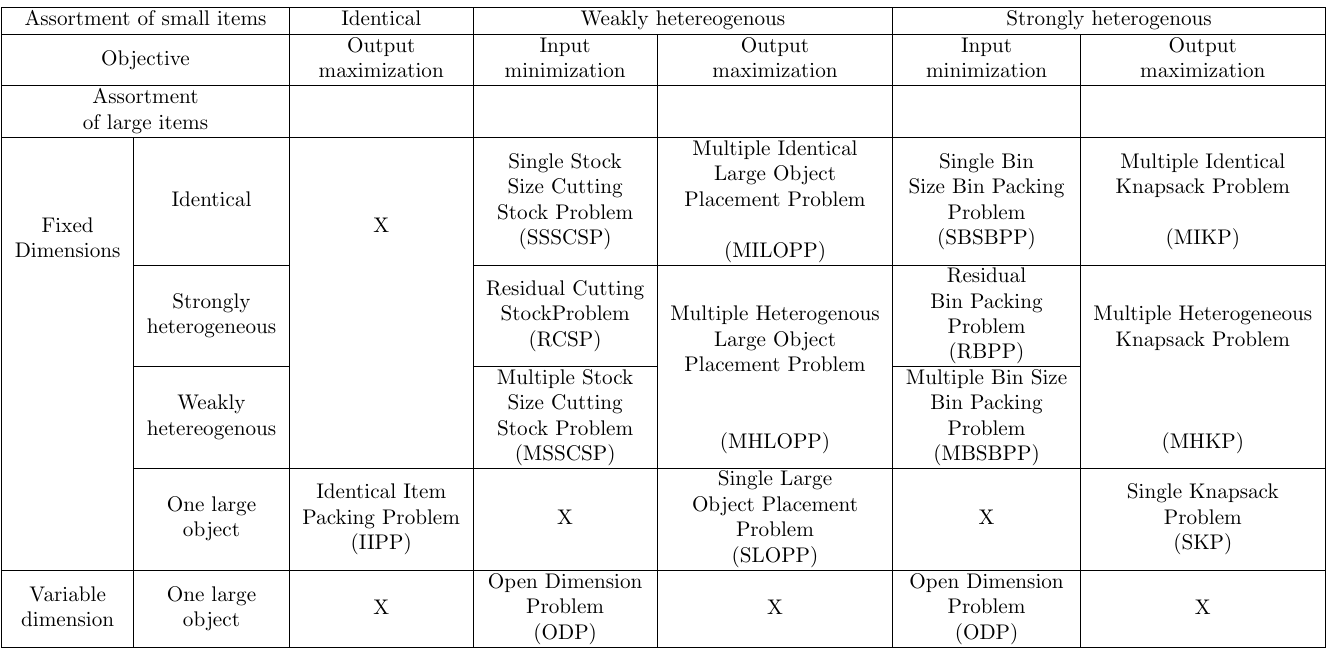
\includegraphics[width=\textwidth]{figures/fig_tab.png}
  % \begin{adjustbox}{width=\textwidth}
  % \begin{tabular}{|cc|c|cc|cc|}
  % \hline
  % \multicolumn{2}{|c|}{Assortment of small items}                                                                                                                          & Identical                                                                             & \multicolumn{2}{c|}{Weakly hetereogenous}                                                                                                                                                                                                                          & \multicolumn{2}{c|}{Strongly heterogenous}                                                                                                                                                                                                              \\ \hline
  % \multicolumn{2}{|c|}{Objective}                                                                                                                                          & \begin{tabular}[c]{@{}c@{}}Output \\ maximization\end{tabular}                        & \multicolumn{1}{c|}{\begin{tabular}[c]{@{}c@{}}Input \\ minimization\end{tabular}}                                       & \begin{tabular}[c]{@{}c@{}}Output\\  maximization\end{tabular}                                                                          & \multicolumn{1}{c|}{\begin{tabular}[c]{@{}c@{}}Input \\ minimization\end{tabular}}                                     & \begin{tabular}[c]{@{}c@{}}Output \\ maximization\end{tabular}                                                                 \\ \hline
  % \multicolumn{2}{|c|}{\begin{tabular}[c]{@{}c@{}}Assortment   \\ of large items\end{tabular}}                                                                             &                                                                                       & \multicolumn{1}{c|}{}                                                                                                    &                                                                                                                                         & \multicolumn{1}{c|}{}                                                                                                  &                                                                                                                                \\ \hline
  % \multicolumn{1}{|c|}{\multirow{4}{*}{\begin{tabular}[c]{@{}c@{}}Fixed\\  Dimensions\end{tabular}}} & Identical                                                           & \multirow{3}{*}{X}                                                                    & \multicolumn{1}{c|}{\begin{tabular}[c]{@{}c@{}}Single Stock \\ Size Cutting \\ Stock Problem \\ (SSSCSP)\end{tabular}}   & \begin{tabular}[c]{@{}c@{}}Multiple Identical \\ Large Object  \\  Placement Problem \\ \\ (MILOPP)\end{tabular}                        & \multicolumn{1}{c|}{\begin{tabular}[c]{@{}c@{}}Single Bin \\ Size Bin Packing \\   Problem\\  (SBSBPP)\end{tabular}}   & \begin{tabular}[c]{@{}c@{}}Multiple Identical \\ Knapsack   Problem \\ \\ (MIKP)\end{tabular}                                  \\ \cline{2-2} \cline{4-7} 
  % \multicolumn{1}{|c|}{}                                                                             & \begin{tabular}[c]{@{}c@{}}Strongly  \\  heterogeneous\end{tabular} &                                                                                       & \multicolumn{1}{c|}{\begin{tabular}[c]{@{}c@{}}Residual Cutting \\ StockProblem \\ (RCSP)\end{tabular}}                  & \multirow{2}{*}{\begin{tabular}[c]{@{}c@{}}Multiple Heterogenous  \\  Large Object\\  Placement Problem \\ \\ \\ (MHLOPP)\end{tabular}} & \multicolumn{1}{c|}{\begin{tabular}[c]{@{}c@{}}Residual \\ Bin Packing \\ Problem   \\ (RBPP)\end{tabular}}            & \multirow{2}{*}{\begin{tabular}[c]{@{}c@{}}Multiple Heterogeneous \\   Knapsack Problem \\ \\ \\ \\ (MHKP)\end{tabular}} \\ \cline{2-2} \cline{4-4} \cline{6-6}
  % \multicolumn{1}{|c|}{}                                                                             & \begin{tabular}[c]{@{}c@{}}Weakly \\   hetereogenous\end{tabular}   &                                                                                       & \multicolumn{1}{c|}{\begin{tabular}[c]{@{}c@{}}Multiple Stock\\  Size Cutting\\  Stock Problem \\ (MSSCSP)\end{tabular}} &                                                                                                                                         & \multicolumn{1}{c|}{\begin{tabular}[c]{@{}c@{}}Multiple Bin Size \\ Bin Packing  \\  Problem \\ (MBSBPP)\end{tabular}} &                                                                                                                                \\ \cline{2-7} 
  % \multicolumn{1}{|c|}{}                                                                             & \begin{tabular}[c]{@{}c@{}}One large  \\  object\end{tabular}       & \begin{tabular}[c]{@{}c@{}}Identical Item\\  Packing Problem   \\ (IIPP)\end{tabular} & \multicolumn{1}{c|}{X}                                                                                                   & \begin{tabular}[c]{@{}c@{}}Single Large \\ Object Placement \\ Problem \\   (SLOPP)\end{tabular}                                        & \multicolumn{1}{c|}{X}                                                                                                 & \begin{tabular}[c]{@{}c@{}}Single Knapsack \\ Problem\\  (SKP)\end{tabular}                                                    \\ \hline
  % \multicolumn{1}{|c|}{\begin{tabular}[c]{@{}c@{}}Variable   \\ dimension\end{tabular}}              & \begin{tabular}[c]{@{}c@{}}One large \\ object\end{tabular}         & X                                                                                     & \multicolumn{1}{c|}{\begin{tabular}[c]{@{}c@{}}Open Dimension\\ Problem \\ (ODP)\end{tabular}}                           & X                                                                                                                                       & \multicolumn{1}{c|}{\begin{tabular}[c]{@{}c@{}}Open Dimension \\ Problem \\ (ODP)\end{tabular}}                        & X                                                                                                                              \\ \hline
  % \end{tabular}
  % \end{adjustbox}
\end{table}


The first mathematical programming model in a scientific journal to describe the container-loading problem was developed in \autocite{Chen1995EUROPEANProblem}, where the authors introduced an MILP model to address the 3D  input minimisation problem by considering rotations and containers of varying dimensions. However, it does not specify the use of weakly or strongly heterogeneous boxes or containers. Additionally, real-world constraints are modelled like, for example, weight distribution.

\autocite{Junqueira2012Three-dimensionalConstraints} propose an alternative MILP formulation to \autocite{Chen1995EUROPEANProblem} using binary encoding for box position, which utilises normal patterns to reduce possible box coordinates by considering multiples of boxes dimensions and ensuring optimal solutions. Additionally, loading and cargo constraints are developed to ensure the static and dynamic stability of the cargo. Boxes must be supported by other box top faces or the container floor. The same authors integrate further loading restrictions in \autocite{Junqueira2012MIP-basedConstraints}, where they integrate multidrop constraints, which address the challenge of packing a
truck with boxes for different customers at various destinations. The goal is to plan the container’s loading to minimise the time spent unloading and reloading boxes at each destination.

\autocite{Zhu2012AProblem} devise a tree search-based method to solve SLOPP and SKP with 3D constraints. Their approach involves evaluating free spaces by employing a look-ahead tree search and selecting optimal placements based on the best free space-block pairs.

\autocite{Goncalves2013AProblems} develop a biased random-key genetic algorithm (BRKGA) designed to solve SBSBPP. The algorithm addresses geometric constraints and introduces a maximal-space representation to handle available free spaces in bins. A novel placement procedure is hybridised with the BRKGA, which optimises the order of box packing and the parameters utilised by the placement procedure to offer an effective solution approach to an NP hard problem.

\autocite{Bortfeldt2013ConstraintsReview} identify constraints for $C\&P$, including item-related constraints (orientation constraints,   load bearing, loading priorities), container-related constraints (weight distribution and weight limit),  and cargo-related constraints (complete-shipment constraints) and load-related constraints ( complexity constraints or stability constraints). The study also highlights the achievements and deficits in container loading research that pertain to these constraints.

\autocite{2016Paquay} propose an MILP model for the MBSBPP.  One noteworthy constraint is the assumption that containers are truncated parallelepiped instead of rectangular boxes. They also consider constraints, such as box rotation, container load bearing, weight distribution, stability and fragility of items.

\autocite{Mahvash2018} introduce a novel resolution procedure for the SBSBPP through the column generation technique, where the columns that are generated are the loading configurations of a single bin. For the pricing develop problem they develop a heuristic to find new columns with a negative reduced cost.  This approach not only produces better results than the previous articles on the literature, but also gives new lower bounds.




\autocite{Silva2019ExactProblems} study SSLOP models with 3D constraints. These authors compare the different approaches that exist in the literature for model packing problems based on two fundamental approaches: discretised formulation \autocite{Junqueira2013AnConstraints} and continuous formulation \autocite{Chen1995EUROPEANProblem} with subsequent modifications. They also indicate that discretised formulation\autocite{Junqueira2012MIP-basedConstraints} performs the best for instances with similar sized boxes. However, it encounters memory limitations for large instances. For other sets of instances, the adapted formulations of \autocite{Chen1995EUROPEANProblem} and \autocite{2016Paquay} outperform other adaptations. Further research topics suggest including the design of new formulations by considering the limited approaches in the literature.



\autocite{Kurpel2020TheProblems} introduce techniques and exact approaches to solve input minimisation and output maximisation problems for container-loading problems. Their methods consider practical constraints, such as orientation, separation of boxes and vertical stability. A set partitioning method is also employed in order to obtain upper bounds in a  container-loading input minimisation problems. The authors adapt and evaluate four discretisation methods found in the existing literature and incorporate mathematical formulations to address the aforementioned constraints.



\autocite{Alonso2020AConstraints} develop an algorithm by the greedy randomised adaptive search procedure (GRASP) to tackle a practical container-loading problem with time-sensitive constraints. Their approach addresses dynamic stability constraints while stacking products on pallets and loading them onto trucks during different time periods. Their approach provides high-quality solutions and surpasses an integer programming formulation in efficiency and effectiveness terms.

\autocite{Ali2022On-lineApproaches} conduct a comprehensive literature review by identifying constraints and solution methods for offline problems with full knowledge of the items to be packed and those tackling the online problems, where items are packed immediately when they arrive, and no prior knowledge of an item is known. The study also identifies and classifies solution approaches for offline packing into six categories: exact methods, constructive heuristics; local search and metaheuristic methods; approximation algorithms; machine learning and hyper-heuristic methods; tree search methods.
\autocite{Harrath2022} proposed a thee stage heuristic based on layer generation to find good quality solutions  the SBSPP problem for large instance up to 993 bins and 200000 items taking into account load balancing constraints.


\autocite{Tresca2022} develop a matheuristic to solve the SBSBPP that includes items with different IDs and different categories, to be delivered to different clients. The algorithm creates monoitem, monocategory, and mixed layers which then are used to compute the final loading configurations of the bins.

\autocite{Li2022} develope a hybrid adaptaive large neighborhood search algoritm to solve the multiple container loading problem, which is tries pack a given set of items with the minimum number of containers while maximazing the space utilization of them. Therfore, it is both a MBSBPP and a MSSCSP. Their approach takes into account some practical applications such as supsension constraints, rotation and weight limit.

\autocite{Chen2023}  present a new approach to the 3D-BPP, introducing the 3D-BSDPP which focuses on optimizing both the design of bin sizes and the packing process. A novel Hybrid Biogeography-Based Optimization (HBBO) algorithm is proposed, integrating differential evolution and a local search strategy for enhanced performance.



One noteworthy trend in $C\&P$ is integrating loading problems with routing. This is known as capacitated vehicle-routing problem with 3D or 2D loading constraints (3L-CVRP or 2L-CVRP). \autocite{Junqueira2012Three-dimensionalConstraints} present a MILP model with binary encodings for 3L-CVRP by including loading, cargo and multidrop constraints. The combination of these two NP-hard problems requires using heuristics and metaheuristics for real-world instances, as seen in \autocite{Dominguez2016UsingFleet}, \autocite{Alonso2022TheRevision} and \autocite{Wei2015AConstraints}. Another noteworthy trend is to use reinforcement learning techniques to solve $C\&P$, as in \autocite{Que2023SolvingLearning} and \autocite{Zhao2022LearningPacking}.


\subsection{Research Gaps \& Methodology}


Here, we discuss the main differences between the 3D-SCPTOP model proposal and those reviewed by specifically focusing on procurement transport. The key distinction of the 3D-SCPTOP model compared to the existing literature is the incorporation of 3D constraints and vertical stability constraints to model transport capacity with a view to providing more realistic solutions and reducing the likelihood of infeasible outcomes.   Table \ref{table:ComProTra}  presents a comparison of inventory modelling, transport modelling, and supply chain configuration between the 3D-SCPTOP model proposal and those currently in the literature.
Hence,  the 3D-SCPTOP approach is based on a SS supply chain configuration, and takes into account the FTL transportation mode.
\begin{table}[h!]
  \begin{adjustbox}{width=\textwidth}
    \begin{tabular}{|c|c|c|c|c|c|c|l|c|c|c|}
      \hline
      Article                                                                            &
      \begin{tabular}[c]{@{}l@{}} SC \\ Configuration\end{tabular}                       &
      \begin{tabular}[c]{@{}l@{}}Decision\\  level\end{tabular}                          &
      \begin{tabular}[c]{@{}l@{}}Transportation \\ Mode\end{tabular}                     &
      \begin{tabular}[c]{@{}l@{}}Transportation \\ Capacity \\   Constraint\end{tabular} &
      \begin{tabular}[c]{@{}l@{}}Transportation\\  Cost\end{tabular}                     &
      \begin{tabular}[c]{@{}l@{}}Inventory\\  Capacity \\ Restriction\end{tabular}       & RTIs           &
      \begin{tabular}[c]{@{}l@{}}Inventory\\  Costs\end{tabular}                         &
      \begin{tabular}[c]{@{}l@{}}Safety \\ Stocks\end{tabular}                           &
      \begin{tabular}[c]{@{}l@{}}Modelling \\ Framework\end{tabular}                                                                                    \\
      \autocite{GUO2024104339}                                                           & MM             & TO & FTL & UH & X & X & S|NF & X &  & MINLP \\\hline \hline
      \autocite{Berman2006InboundCost}                                                   &
      MM                                                                                 &
      T                                                                                  &
      FTL|LTL                                                                            &
      V                                                                                  &
      X                                                                                  &
                                                                                         &                &
      X                                                                                  &
                                                                                         &
      MINLP                                                                                                                                             \\ \hline
      \autocite{Sancak2011Multi-itemPolicy}                                              &
                                                                                         &
      O                                                                                  &
      LTL|FTL                                                                            &
      V                                                                                  &
      X                                                                                  &
                                                                                         &                &
      X                                                                                  &
      X                                                                                  &
      MILP                                                                                                                                              \\ \hline
      \autocite{Schoneberg2010AnNetworks}                                                &
      MS                                                                                 &
      T                                                                                  &
      FTL|LTL                                                                            &
      V                                                                                  &
      X                                                                                  &
      X                                                                                  &                &
      X                                                                                  &
                                                                                         &
      MILP                                                                                                                                              \\ \hline
      \autocite{Schoneberg2013ANetworks}                                                 &
      MS                                                                                 &
      O                                                                                  &
      FTL|LTL                                                                            &
      V                                                                                  &
      X                                                                                  &
      X                                                                                  &                &
      X                                                                                  &
                                                                                         &
      MILP                                                                                                                                              \\ \hline
      \autocite{Diaz-Madronero2014APlanning}
                                                                                         &
      SS                                                                                 &
      O                                                                                  &
      FTL                                                                                &
      UH                                                                                 &
      X                                                                                  &
                                                                                         &                &
      X                                                                                  &
      X                                                                                  &
      FMOILP                                                                                                                                            \\ \hline
      \autocite{Hein2016QuantitativeProblem}                                             &
      MS                                                                                 &
      O                                                                                  &
      MR                                                                                 &
      V                                                                                  &
      X                                                                                  &
                                                                                         &                &
      X                                                                                  &
                                                                                         &
      MILP                                                                                                                                              \\ \hline
      \autocite{Diaz-Madronero2017ADecisions}                                            &
      MS                                                                                 &
      T                                                                                  &
      FTL|LTL|MR                                                                         &
      V                                                                                  &
      X                                                                                  &
      X                                                                                  &                &
      X                                                                                  &
      X                                                                                  &
      MILP                                                                                                                                              \\ \hline
      \autocite{Meyer2018TransportIndustry}                                              & MS
                                                                                         & T|O
                                                                                         & MR|FTL
                                                                                         & V
                                                                                         & X
                                                                                         & X
                                                                                         &                & X
                                                                                         &
                                                                                         & MILP
      \\ \hline
      \autocite{Chitsaz2019ARouting}                                                     &
      MS                                                                                 &
      O|T                                                                                &
      MR                                                                                 &
      V                                                                                  &
      X                                                                                  &
      X                                                                                  &                &
      X                                                                                  &
                                                                                         &
      MILP                                                                                                                                              \\ \hline
      \autocite{Baller2022OptimizingApproach}                                            & MS
                                                                                         & O
                                                                                         & MR|FTL|LTL|CES
                                                                                         & V|W
                                                                                         & X
                                                                                         & X
                                                                                         &                &
                                                                                         & X
                                                                                         & MILP
      \\ \hline
      \autocite{Hashemi-Amiri2023IntegratedApproach}                                     &
      MS                                                                                 &
      T                                                                                  &
      MR                                                                                 &
      V                                                                                  &
      X                                                                                  &
                                                                                         &                &
                                                                                         &
                                                                                         &
      CCP                                                                                                                                               \\ \hline
      3D-SCPTOP                                                                          &
      SS                                                                                 &
      O                                                                                  &
      FTL                                                                                &
      3D-Constraints                                                                     &
      X                                                                                  &
      X                                                                                  &                &
      X                                                                                  &
      X                                                                                  &
      MILP                                                                                                                                              \\ \hline
      \autocite{Zhang17012024}                                                           & MS             & TO & MR  & UH & X & X & M|NF & X &  & ILP   \\\hline
    \end{tabular}
  \end{adjustbox}
  \begin{tablenotes}
    \scriptsize
    \item  \textbf{Abbreviations.}  \textbf{T} (tactical), \textbf{O} Operational; \textbf{FTL} (full-truck load), \textbf{LTL} (less-than-truck load), \textbf{MR} (milk-run), \textbf{CES} (courier express service); \textbf{V} (volumetric), \textbf{W} (weight), \textbf{UH} Unit Holding;   \textbf{CCP} chance-constrained programming
  \end{tablenotes}
  \caption{Comparison of procurement transport models}
  \label{table:ComProTra}
\end{table}

On the other hand, the 3D-SCTOP model diverges from those proposed in the packaging literature in several aspects. Firstly, the loading problem takes into account different time periods. Therefore, the specific container (small items or boxes in the $C\&P$ literature) that we utilise are yet to be defined, as the choice of container depends on the inventory levels of each product.
Also, the objective function depends on inventory and transport costs, which are inherently connected to the loading problem at hand. Thefore, we simultaneously solve an input minimisation  and output maximisation problem. Both of these are a result of transport minimisation and inventory costs. Input minimisation comes because we want to find the minimum number of trucks needed. Meanwhile, output maximization comes from the FTL and the transport costs.

\begin{table}
  \begin{adjustbox}{width=\textwidth}
    \begin{tabular}{|c|c|c|c|c|c|c|c|} \hline
      Article                           & Problem type     & Resolution procedure & Orientation & Weight & Load Balance & Stability & Time-Depenent \\
      \hline
      \autocite{Zhu2012AProblem}        & SLOP|SKP         & TSM                  & X           & X      &              &           &               \\ \hline
      \autocite{Goncalves2013AProblems} & SBSBPP           & BRKGA                & X           & X      &              & X         &               \\ \hline
      \autocite{2016Paquay}             & SBSBPP           & EM                   & X           & X      & X            & X         &               \\ \hline
      \autocite{Mahvash2018}            & SBSBPP           & CG                   & X           & X      &              &           &               \\ \hline \autocite{Alonso2020AConstraints}& SSSCSP& GRASP& X& X& X& X&X\\ \hline
      \autocite{Tresca2022}             & SBSBPP           & MH                   & X           & X      & X            & X         &               \\ \hline
      \autocite{Harrath2022}
                                        & SBSBPP           & H                    & X           & X      & X            &           &               \\ \hline
      \autocite{Li2022}                 & SBSBPP|MSSCSP    & HALNs                & X           & X      &              & X         &               \\
      \hline
      \autocite{Chen2023}               & BSDPP            & HBBO                 & X           & X      &              &           &               \\
      \hline
      3D-SCPTOP                         & SSSCSP \& MILOPP & MH                   & X           & X      & X            & X         & X             \\ \hline
    \end{tabular}
  \end{adjustbox}
  \begin{tablenotes}
    \scriptsize
    \item  \textbf{Abbreviations.}  \textbf{T}SM (Tree search method), \textbf{BRKGA} Biased Randomized Jey Genetic Algorithm; \textbf{EM} (Exact Metods), \textbf{MH} (MatHeuristic), \textbf{CG} (Column Generation), \textbf{H} (Heuristic); \textbf{HCLP} (Hybrid Adaptive Large Neighborhood Search), \textbf{HBBO} (Hybrid Biogeography-Based Optimization)
  \end{tablenotes}
  \label{tab:my_label}
  \caption{Comparison of C\&P problems}
\end{table}

% \begin{figure}
%     \centering
%     \includegraphics[scale=0.5]{FiguraPaperv2-cropped.pdf}
%     \caption{Caption}
%     \label{fig:enter-label}
% \end{figure}


Based on the literature review and the identified research gaps, our proposal is structured according to the steps depicted in Figure \ref{fig:tikz1}.

\begin{figure}[h!]
  \centering
  \resizebox{0.85\columnwidth}{!}{
    \begin{tikzpicture}[node distance=2cm, auto, thick]

      % Define styles
      \tikzstyle{block} = [rectangle, draw, fill=blue!40, text width=14em, text centered,  minimum height=3em]
      \tikzstyle{sideblock} = [rectangle, draw, fill=white, text width=10em, text centered, rounded corners, minimum height=2em]
      \tikzstyle{grayblock} = [rectangle, draw, fill=gray!20, text width=13em, text centered, rounded corners, minimum height=2.5em]
      \tikzstyle{line} = [draw, -Latex]
      \tikzstyle{plainline} = [draw]
      \tikzstyle{dashedline} = [draw, dashed, gray, thick, -Latex]





      % Central nodes
      \node [block] (literature) {Literature Review};
      \node [grayblock, below=0.35cm of literature] (research) {Research Gap};
      \node [block, below=0.35cm of research] (problem) {Problem Statement};
      \node [grayblock, below=0.35cm of problem] (3dMilp) {3D-SCPTOP};
      \node [grayblock, below=0.35cm of 3dMilp] (3dMH) {MH-3D-SCPTOP};
      \node [block, below=0.35cm of 3dMH] (experiments) {Computational Experiments};
      \node [grayblock, below=0.35cm of experiments] (procedure) {Resolution \\ Procedure Comparison};
      \node [grayblock, below=0.35cm of procedure] (comparison) {Model Comparison};
      \node[ aux_gene_group,fit=(comparison) (procedure)] (gr1) {};

      \node [block, below=0.35cm of comparison] (case) {Case Study \& \\ Managerial Implications};

      % Side nodes
      \node [sideblock, above=1cm of literature] (model) {Modelling \& \\ Resolution Appoach};
      \node [sideblock, left=1cm of literature] (procurement) {Procurement Transport};
      \node [sideblock, right=1cm of literature] (3D) {3D Container Loading};

      % Draw edges for side nodes (with dashed gray lines and arrows)
      \path [dashedline] (3D) -- (literature);
      \path [dashedline] (model) -- (literature);
      \path [dashedline] (procurement) -- (literature);

      % Side nodes
      \node [sideblock, left=1cm of 3dMH] (MILP) {MILP};
      \node [sideblock, right=1cm of 3dMH] (MetaHeuristic) {Metaheuristic};

      % Draw edges for side nodes (with dashed gray lines and arrows)
      \path [dashedline] (MILP) -- (3dMH);
      \path [dashedline] (MetaHeuristic) -- (3dMH);

      % % Side nodes
      % \node [sideblock, above left=1.25cm and 1cm of comparison] (small) {Small Instances};
      % \node [sideblock, below=0.5cm of small] (medium) {Medium Instances};
      % \node [sideblock, below=0.5cm of medium] (large) {Large Instances};

      % Side nodes
      \node [sideblock, left=0.5cm of gr1] (medium) {Medium Instances};

      \node [sideblock, above=0.5cm of medium] (small) {Small Instances};
      \node [sideblock, below=0.5cm of medium] (large) {Large Instances};

      \coordinate (center13) at ($(procedure.west)!1/3!(procedure.south west)$);
      \coordinate (center12) at ($(procedure.west)$);
      \coordinate (center23) at ($(procedure.west)!2/3!(procedure.north west)$);


      % Draw edges for side nodes (with dashed gray lines and arrows)
      \path [dashedline] (small.east) -- (center23) ;
      \path [dashedline] (medium.east)  -- (center12) ;
      \path [dashedline](large.east)  -- (center13) ;


      \coordinate (ccenter13) at ($(comparison.west)!1/3!(comparison.south west)$);
      \coordinate (ccenter12) at ($(comparison.west)$);
      \coordinate (ccenter23) at ($(comparison.west)!2/3!(comparison.north west)$);


      % Draw edges for side nodes (with dashed gray lines and arrows)
      \path [dashedline] (small.east) -- (ccenter23) ;
      \path [dashedline] (medium.east)  -- (ccenter12) ;
      \path [dashedline](large.east)  -- (ccenter13) ;




      % Draw edges for central nodes and gray nodes
      \path [plainline] (literature)  -- (research);
      \path [line] (research) -- (problem);
      \path [plainline] (problem)  -- (3dMilp);
      \path [plainline] (3dMilp)  -- (3dMH);
      \path [line] (3dMH) -- (experiments);
      \path [plainline] (experiments)  -- (procedure);
      \path [plainline] (procedure)  -- (comparison);
      \path [line] (comparison) -- (case);






      % Side nodes
      \node [sideblock, right=1cm of comparison] (reference) {With respect \autocite{Diaz-Madronero2014APlanning}};

      % Draw edges for side nodes (with dashed gray lines and arrows)
      \path [dashedline] (reference) -- (comparison);







    \end{tikzpicture}
  }
  \caption{Research Methodology}
  \label{fig:tikz1}
\end{figure}

\FloatBarrier




\section{Problem Description}
The main objective of the presented problem is to minimise the transportation and inventory holding costs of a manufacturing site by integrating procurement transport, RTI management and inventory decisions with 3D full-truck loading constraints. The supply chain under study has a single source and a single destination. FTL is employed as the mode of transport. Products are shipped in different RTI types. RTIs are transported inside trucks, and the loading configuration is determined. Therefore, a distinction is made to the classic nomenclature of $C\&P$ problems. Hereafter, small objects are RTIs and large objects are trucks.

The assembler’s demand drives the procurement process because it determines the optimal quantity of the products to procure from the supplier to the manufacturing site. Raw materials and assembled parts are produced at the supplier following the production plan. Then, they are packed in their corresponding RTI. The full RTIs with RM and AP are transported using an FTL mode of transport with 3D loading constraints. Each RTI can only carry the same product type at a given time.
Furthermore, each RM or AP can only be shipped in one RTI type. Once the full RTIs are at the plant, the RM and AP are used for production, and the RTIs are emptied. Once emptied, they are folded and shipped back to the supplier using FTL transport with 3D loading constraints. Figure \ref{fig:FormulacionContenedor} is an example of the assignment of RM and AP to RTI types, where three container types and six product types are represented in different colours. The arrow indicates the amount of product that can be shipped in the containers.


\begin{figure}[h!]
  \centering
  % 
\includegraphics[scale=0.25]{fig_container_formulation.png}
  \input{vistex/product_box_vis}

  \caption{Product to type of reusable container}
  \label{fig:FormulacionContenedor}
\end{figure}
\FloatBarrier
In our problem, two distinct transport decisions are made: procuring RM and AP for the manufacturing plant with full RTIs. And the supply of empty RTIs to the supplier.
\begin{figure}[h!]
  \centering
  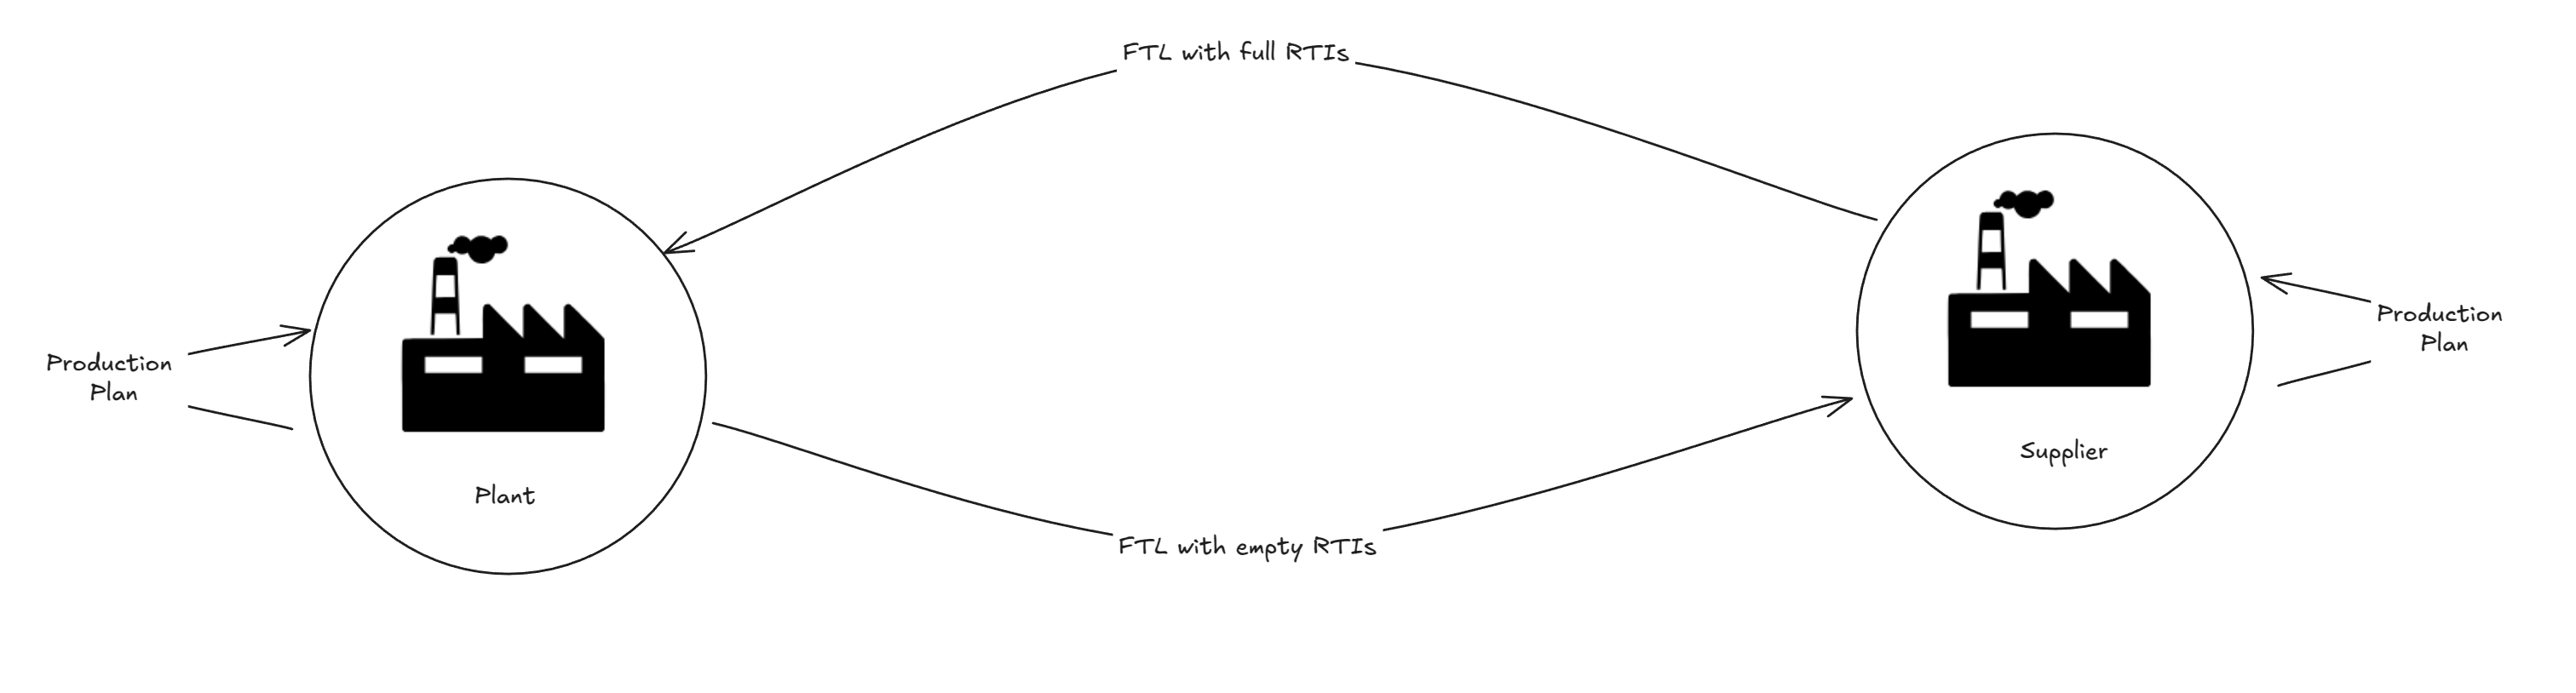
\includegraphics[width=0.75\linewidth]{figures/SupplyChain.png}
  \caption{Enter Caption}
  \label{fig:enter-label}
\end{figure}

\begin{figure}
  \centering
  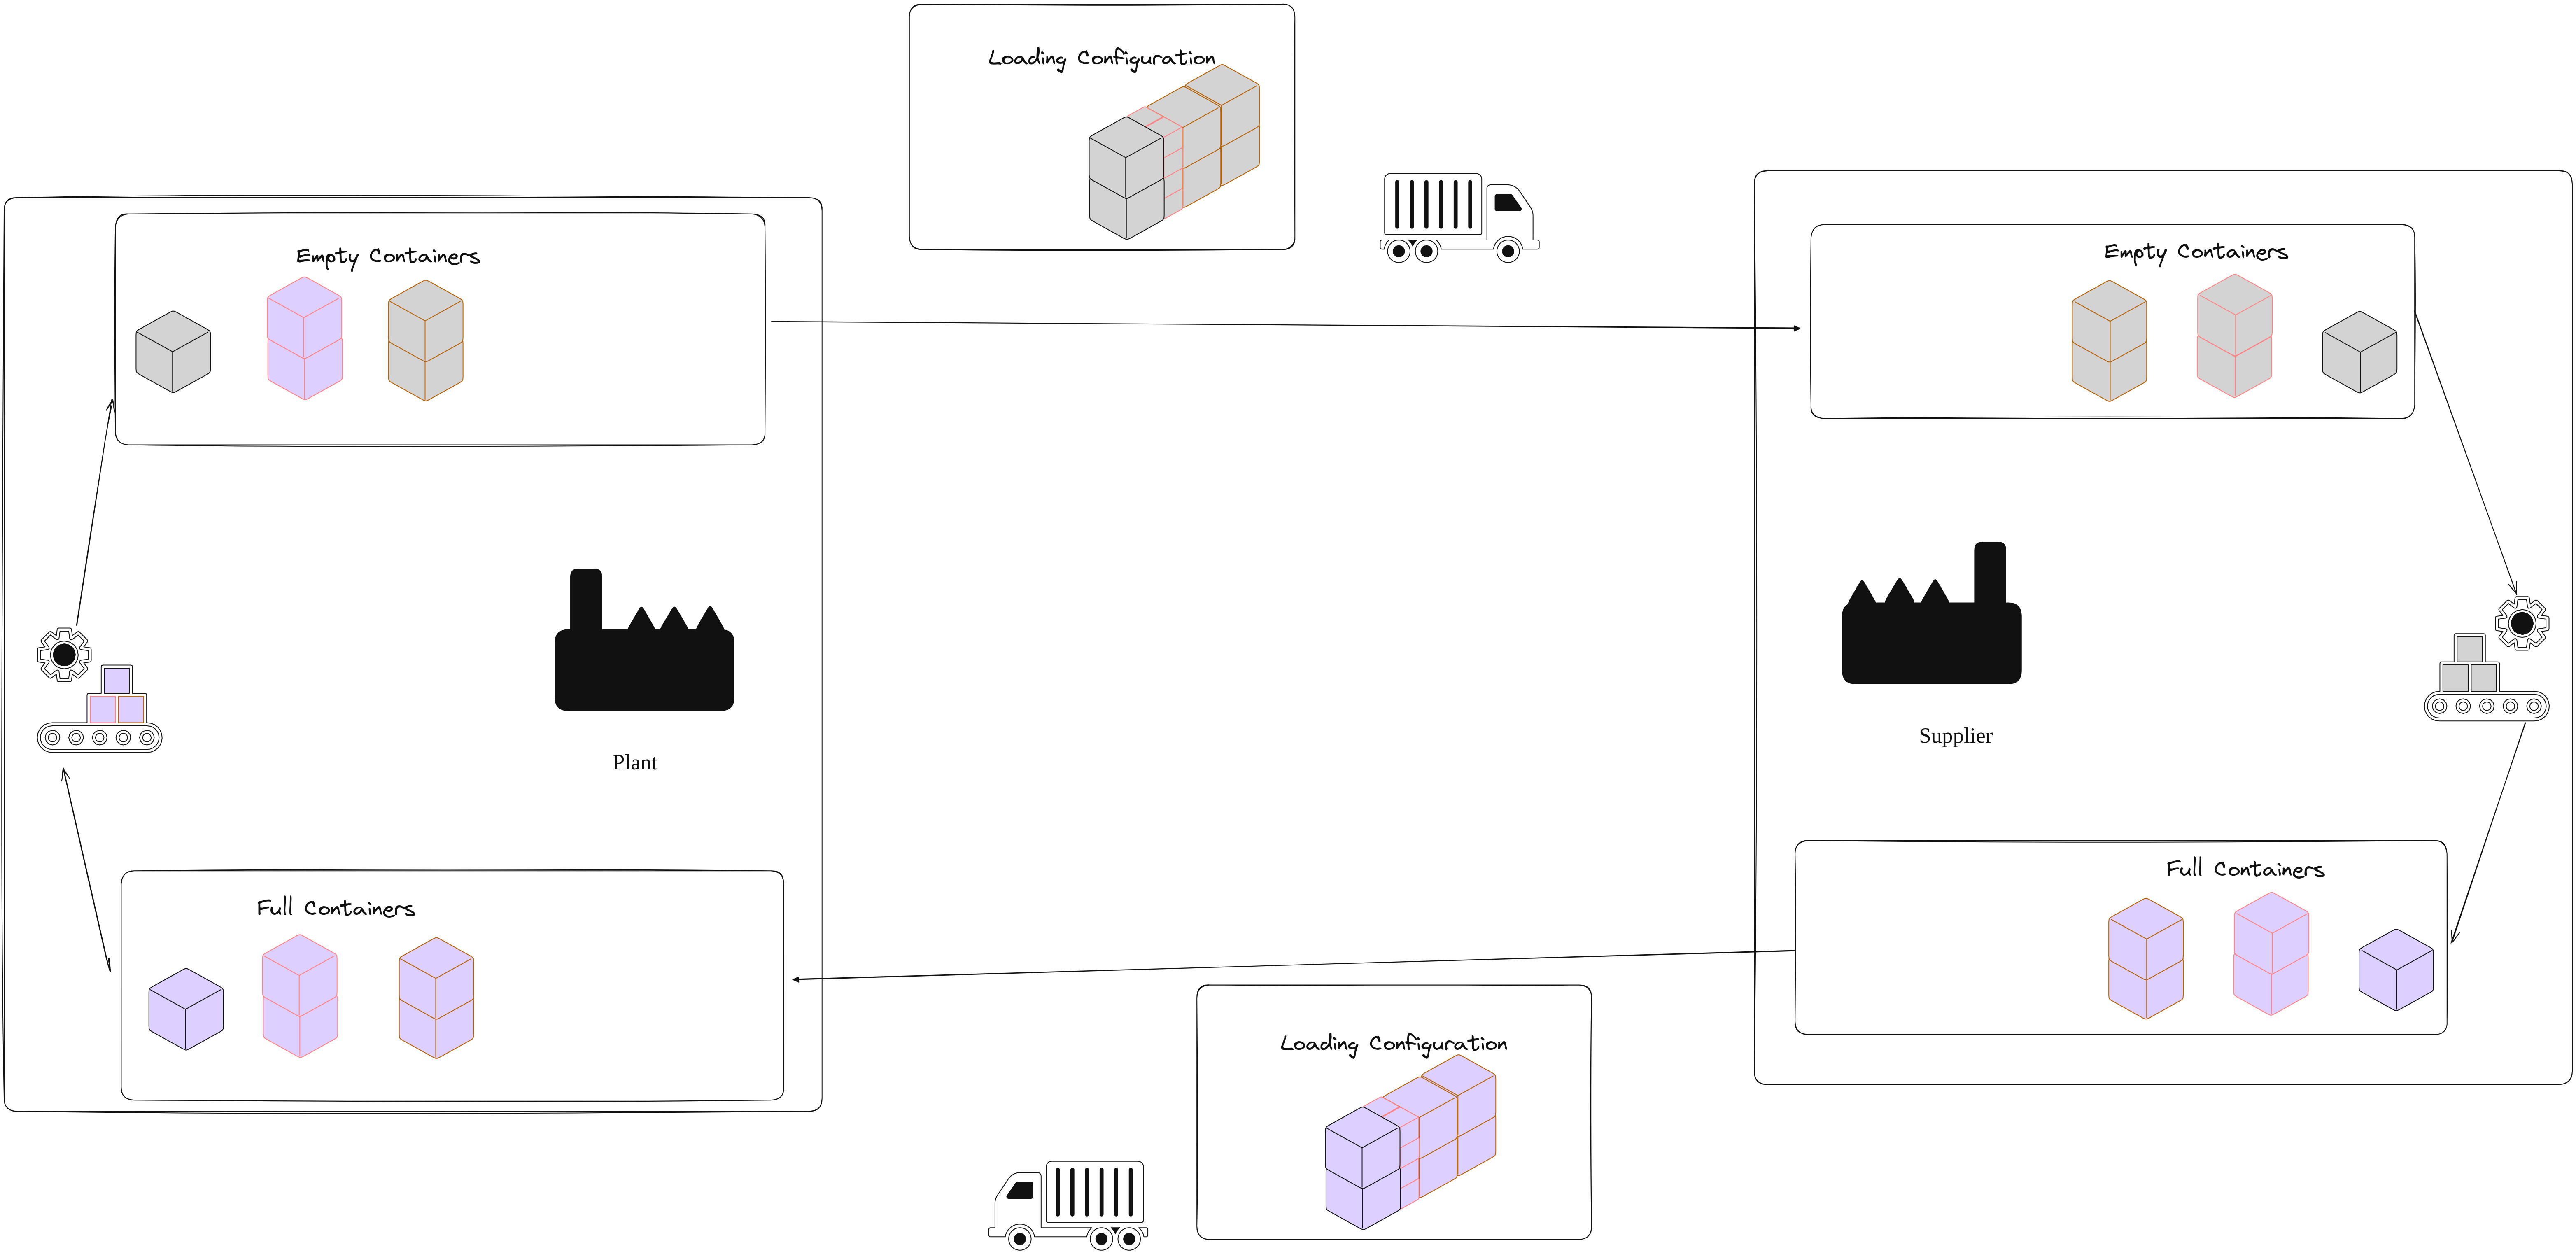
\includegraphics[width=0.5\linewidth]{figures/Untitled-2025-03-24-0935.png}
  \caption{Enter Caption}
  \label{fig:enter-label}
\end{figure}

Several constraints and assumptions are considered in this model formulation. Firstly, the physical transport constraints ensure that RTIs do not overlap and are contained in the truck. A truck’s maximum weight limit must not be exceeded. Maintaining the static stability of containers during transport is crucial to prevent tipping or shifting because it could damage RM and AP. Rotations of containers about z-axes are allowed. As FTL is the mode of transport employed, trucks should be loaded to achieve a minimum utilisation percentage. Furthermore, we assume that the supplier's production plans and the plan are synchronised to guarantee the production of the manufacturing site. Minimum inventory coverage constraints are considered, subject to the product’s future demand.
Thus, the problem can be formulated in the following way:


\textbf{Initial data:}
\begin{itemize}
  \item Product data: initial inventory, demand for each time period of the plant in terms of full RTIs, the type of reusable container in which it must travel, production demand for each time period at the supplier in terms of RTIs, and the weight of the RTI when loaded with the given product
  \item Reusable container data: RTI dimensions when full and folded.
  \item Transport data: number of available trucks, minimum utilisation percentage, dimensions and maximum weight
\end{itemize}
\textbf{To determine:}
\begin{itemize}
  \item The number of trucks used daily with their corresponding loading configuration.
  \item The inventory level in terms of full RTIs for each product in the factory and supplier, given that everything goes according to plan.
  \item The inventory level of folded RTIs in the factory and supplier.
\end{itemize}
\textbf{Subject to:}
\begin{itemize}
  \item Loading restrictions (i,e: containers cannot overlap, rotations about z axes are allowed, the maximum weight of a truck can not be exceeded, static stability)
  \item Minimum coverage stock
\end{itemize}
\textbf{In order to:}
\begin{itemize}
  \item Minimise the total transportation cost
  \item Minimise the total inventory holding cost
\end{itemize}

\section{Mathematical model}
The 3D-SCPTOP mathematical programming model integrates container loading constraints and procurement transport decisions. It differs from  traditional 3D container packing problems in two significant aspects. Firstly, the quantity of containers required for loading depends on product demand and the inventory levels of the manufacturing site. Therefore, the specific products to be transported are identified to minimise transport and inventory costs. As inventory levels depend on past loading decisions, a time dimension has to be taken into account. Secondly, it combines output maximisation problems and input minimisation. On the one hand, the number of trucks to be used is minimised, i.e. input minimisation. On the other hand, trucks must be fully loaded, i.e. output maximisation. It also extends traditional procurement transport planning approaches by taking into account 3D loading constraints and RTI management.


Table \ref{tab:Nomenclature} presents the nomenclature of the 3D-SCPTOP model.
\FloatBarrier
\begin{longtable}[hbt!]{  |p{0.13\textwidth}|p{0.85\textwidth}  |}
  \caption{Nomenclature of 3D-SCPTOP}
  \label{tab:Nomenclature}
  \\
  \hline
  \multicolumn{2}{|l|}{\textbf{Indices}}                                                                                                                                                                                                                                                                                                                                                                                                                                                                                                                                                                                                                                          \\ \hline
  $R$                                                                                            & Set of RTI types $(r = 1, \dots, R)$                                                                                                                                                                                                                                                                                                                                                                                                                                                                                                                                           \\
  $I$                                                                                            & Set of RTIs $(i = 1, \dots , I)$                                                                                                                                                                                                                                                                                                                                                                                                                                                                                                                                               \\
  $K$                                                                                            & Set of trucks $(k =1,\dots , K)$
  \\
  \textit{N}                                                                                     & Set of products $(n =   1,\dots,N)$                                                                                                                                                                                                                                                                                                                                                                                                                                                                                                                                            \\
  $L$                                                                                            & Set of loading configurations $(l =1,2,\dots , L)$
  \\
  \textit{T}                                                                                     & Set of planning periods \textit{(t} =1, \dots \textit{T)}                                                                                                                                                                                                                                                                                                                                                                                                                                                                                                                      \\
  $G$                                                                                            & Set corresponding to the supplier and plant nodes $G = \lbrace s, p \rbrace$                                                                                                                                                                                                                                                                                                                                                                                                                                                                                                   \\
  \hline
  \multicolumn{2}{|l|}{\textbf{Set of indices}}                                                                                                                                                                                                                                                                                                                                                                                                                                                                                                                                                                                                                                   \\ \hline
  $M(r)$                                                                                         & Set of RM or AP that are carried in RTI $r \in R$, $n = 1, \dots, M(r)$                                                                                                                                                                                                                                                                                                                                                                                                                                                                                                        \\
  \hline
  \multicolumn{2}{|l|}{\textbf{Parameters}}                                                                                                                                                                                                                                                                                                                                                                                                                                                                                                                                                                                                                                       \\ \hline
  $cK$                                                                                           & Cost of using a truck                                                                                                                                                                                                                                                                                                                                                                                                                                                                                                                                                          \\
  $lt$                                                                                           & Lead transport time between the plant and the supplier and viceversa.                                                                                                                                                                                                                                                                                                                                                                                                                                                                                                          \\
  \textit{$i_{gn}$}                                                                              & Initial inventory level of $n\in N$ in $g \in G$ in terms of full RTIs                                                                                                                                                                                                                                                                                                                                                                                                                                                                                                         \\
  \textit{$ie_{gr}$}                                                                             & Initial inventory level of empty RTIs $r\in R$ in $g \in G$ RTIs                                                                                                                                                                                                                                                                                                                                                                                                                                                                                                               \\
  \textit{$ic_{gn}$}                                                                             & Inventory cost of $n\in N$ at $g \in G$ in terms of full RTIs                                                                                                                                                                                                                                                                                                                                                                                                                                                                                                                  \\
  $d_{gnt}$                                                                                      & Production plan of $n \in N$ at $g \in G$ during time period $t\in T$                                                                                                                                                                                                                                                                                                                                                                                                                                                                                                          \\
  $q_{rt}$                                                                                       & Initial quantity of empty RTIs $r\in R$ arriving at supplier $s\in G$ in time period $t \in (1,\dots , lt)$                                                                                                                                                                                                                                                                                                                                                                                                                                                                    \\
  $q_{nt}$                                                                                       & Initial quantity of full RTIs of $n \in R$ arriving at $p$ in time period $t \in (1,\dots , lt)$                                                                                                                                                                                                                                                                                                                                                                                                                                                                               \\
  $lc_{lrg}$                                                                                     & Number of containers of type $c$ used in loading configuration $l$ arriving at $g\in G$                                                                                                                                                                                                                                                                                                                                                                                                                                                                                        \\
  $ss_{gnt}$                                                                                     & Security stock for product $n\in N$  in time period $t \in T$ in $g \in G$ in terms of full RTIs                                                                                                                                                                                                                                                                                                                                                                                                                                                                               \\
  $ss_{gtr}$                                                                                     & Security stock of empty RTIs $r\in R$  in time period $t \in T$ in $g \in G$                                                                                                                                                                                                                                                                                                                                                                                                                                                                                                   \\
  \textit{$w_{n}$}                                                                               & Weight of a container carrying product \textit{n}
  \\
  \textit{$pK$}                                                                                  & Maximum  weight capacity of a truck                                                                                                                                                                                                                                                                                                                                                                                                                                                                                                                                            \\
  \textit{$pK$}                                                                                  & Maximum  weight capacity of truck a truck                                                                                                                                                                                                                                                                                                                                                                                                                                                                                                                                      \\
  \textit{$\Gamma_c$}                                                                            & Volume of a container type $c$                                                                                                                                                                                                                                                                                                                                                                                                                                                                                                                                                 \\
  \textit{$\Gamma$}                                                                              & Volume of a truck                                                                                                                                                                                                                                                                                                                                                                                                                                                                                                                                                              \\
  \textit{$\alpha$}                                                                              & Minimum volume utilisation of a truck                                                                                                                                                                                                                                                                                                                                                                                                                                                                                                                                          \\
  \textit{M}                                                                                     & A large enough number to make the logic of the model work;                                                                                                                                                                                                                                                                                                                                                                                                                                                                                                                     \\
  $p_{gr}, q_{gr}, r_{gr}$                                                                       & length, width, and height of a container of type c;                                                                                                                                                                                                                                                                                                                                                                                                                                                                                                                            \\
  $p{K}, q{K}, r{K}$                                                                             & Length, width and height of a truck;                                                                                                                                                                                                                                                                                                                                                                                                                                                                                                                                           \\[0.15cm]
  \hline
  \multicolumn{2}{|l|}{\textbf{Decision Variables}}                                                                                                                                                                                                                                                                                                                                                                                                                                                                                                                                                                                                                               \\ \hline
  $I_{gnt}$                                                                                      & Inventory of product $n\in N$ at the end of $t\in T$ time period at $g\in G$ in terms of full RTIs                                                                                                                                                                                                                                                                                                                                                                                                                                                                             \\
  $Ie_{gtr}$                                                                                     & Inventory of empty RTIs $r\in R$ at the end of $t\in T$ time period at $g\in G$                                                                                                                                                                                                                                                                                                                                                                                                                                                                                                \\
  $Y_{gkt}$                                                                                      & Binary variable, if one then  truck $k \in K$ is used in time period $t\in T$ arriving at $g\in G$ and zero otherwise                                                                                                                                                                                                                                                                                                                                                                                                                                                          \\
  $Y_{gklt}$                                                                                     & Binary variable, if one then truck $k \in K$ is used in time period $t\in T$ departing from $g\in G$ using loading configuration $l$, 0 otherwise                                                                                                                                                                                                                                                                                                                                                                                                                              \\
  $Q_{nt}$                                                                                       & Integer variable indicating the number of RM or AP $n\in N$ in transport during time period $t$ to the manufacturing plant $p$                                                                                                                                                                                                                                                                                                                                                                                                                                                 \\
  $Q_{rt}$                                                                                       & Integer variable the number of empty RTIs $r\in R$ in transport during time period $t$ to the supplier $s$                                                                                                                                                                                                                                                                                                                                                                                                                                                                     \\
  $V_{gklrt}$                                                                                    & Number of RTIs $r\in R$ in truck $k\in K$ using loading configuration $l\in L$ at time period $t\in T$ departing from $g\in G$                                                                                                                                                                                                                                                                                                                                                                                                                                                 \\
  $V_{kglnt}$                                                                                    & Number of full RTIs with RM or AP $n\in N$ in truck $k\in K$ using loading configuration $l\in L$ at time period $t\in T$ departing from $g\in G$                                                                                                                                                                                                                                                                                                                                                                                                                              \\
  \textit{I$_{nt}$}                                                                              & Inventory of product \textit{n} at the end of  time period  \textit{t}                                                                                                                                                                                                                                                                                                                                                                                                                                                                                                         \\[0.15cm]
  \textit{$X_{gil}$}                                                                             & Binary variable indicating whether container \textit{i} is used in loading configuration \textit{l}                                                                                                                                                                                                                                                                                                                                                                                                                                                                            \\[0.15cm]
  \textit{$X_{gilr}$}                                                                            & Binary variable indicating whether container \textit{i} is going to be of type \textit{c} for loading configuration \textit{l}                                                                                                                                                                                                                                                                                                                                                                                                                                                 \\[0.15cm]
  \textit{$V_{gklrt}$}                                                                           & Number of containers of type $c$ in truck $k$ using loading configuration $l$ at time period $t$                                                                                                                                                                                                                                                                                                                                                                                                                                                                               \\[0.15cm]
  \textit{$V_{kglnt}$}                                                                           & Integer variable indicating the quantity of containers carrying product \textit{n} supplied on truck \textit{k} using loading configuration $l$ at time period $t$.                                                                                                                                                                                                                                                                                                                                                                                                            \\[0.15cm]
  \textit{$PX_{gil},$ $PY_{gil},$ $PZ_{gil}$}                                                    & Coordinates of the lower left front corner of container \textit{i} on the truck \textit{k} during planning period \textit{t};                                                                                                                                                                                                                                                                                                                                                                                                                                                  \\[0.15cm]
  \textit{$LX_{gilr},LY_{gilr}$ $,LZ_{gilr}$}                                                    & Defines whether the length of container \textit{i} of type c is on the same direction as the x-, y- or z-axis in loading configuration $l$. For example, $LX_{gilr}$ equals one if the length of container \textit{i} of type c is is on the same direction as the x-axis, otherwise $LX_{gilr}$ equals 0;                                                                                                                                                                                                                                                                     \\[0.15cm]
  $WX_{gilr}$ $,WY_{gilr}$ $,WZ_{gilr}$                                                          & Defines whether the width of container \textit{i} of type c is on the same direction as the x-, y- or z-axis on truck \textit{k} axis during planning period \textit{t}. For example, $WX_{gilr}$ equals 1 if the width of  container \textit{i} of type c is is on the same direction as the x-axis, otherwise $WX_{gilr}$ equals 0;                                                                                                                                                                                                                                          \\[0.25cm]
  \textit{$HX_{gilr}, $ $ HY_{gilr}$ $,HZ_{gilr}$}                                               & Defines whether the height of container \textit{i} of type c is on the same direction as the x-, y- or z-axis on the truck \textit{k} axis during planning period \textit{t}. For example, $HX_{gilr}$ equals 1 if the width of container \textit{i} of type c is is on the same direction as the x-axis, otherwise $HX_{gilr}$ equals 0                                                                                                                                                                                                                                       \\[0.15cm]
  $A_{g i j l}, $ $ B_{g i j l}, $ $C_{g i j l}, $ $ D_{g i j l},$ $E_{g i j l}, $ $F_{g i j l}$ & Binary variables indicating the relative position between two boxes. Variable $A_{g i j l}$ equals 1 if container \textit{i} is to the left of container j on truck \textit{k} during planning period \textit{t}. Similarly, variables $B_{g i j l}$,$C_{g i j l}$$, D_{g i j l}$ $, E_{g i j l}$ $, F_{g i j l}$ indicate whether container \textit{i} is to the right, behind, in front, on top or below container \textit{j}, respectively, on truck \textit{k} during planning period \textit{t}. These variables are only necessary when \textit{i} $\not = $ \textit{k}. \\[0.15cm]
  \hline
\end{longtable}

\FloatBarrier

{We wish to minimise the total cost, which is given by  transportation and inventory costs.}
\begin{equation}
  \text{\textit{Min} } z= \sum_{g \in G}{\sum_{k \in K}{\sum_{t \in T}{Y_{gkt}\cdot cK}}}+ \sum_{g \in G}{\sum_{n \in N}{\sum_{t \in T}{I_{gnt}\cdot ic_{gn}}}}
\end{equation}


\eqref{eq:1PLC} - \eqref{eq:2PLC}  define the inventory level of RM or AP according to the production demand and supply of RM or AP  from the supplier $s$ at the plant  $p$
\begin{align}
  I_{pnt}  & =I_{pnt^{\prime}}-d_{pnt}+Q_{nt^{\prime}}\quad             & \forall n \in N,t \in T : t\ge    lt +1,t^{\prime}\coloneqq t-lt \label{eq:1PLC} \\
  I_{pnt}  & =I_{pnt'}-d_{pnt}+q_{nt}\quad                              & \forall n \in N,t \in (2,\dots, lt) : ,t^{\prime}\coloneqq t-lt\label{eq:3PLC}   \\
  I_{pnt}  & =i_{pn}-d_{pnt}+q_{nt}\quad                                & \forall n \in N: t \coloneqq 1 \label{eq:2PLC}                                   \\
  Ie_{ptr} & =Ie_{pt^{\prime}r}+\sum_{n \in M(r)}{d_{pnt}}-Q_{rt} \quad & \forall r \in R,t \in T : t\ge 2                                                 \\
  Ie_{ptr} & =ie_{pr}+\sum_{n \in M(r)}{d_{pnt}}-Q_{rt}\quad            & \forall r \in R , t\coloneqq 1
\end{align}
\eqref{eq:1PLC-s} - \eqref{eq:2PLC-s}  the empty RTIs according to the production demand and supply of RTIs from the plant $p$ at the supplier $s$
\begin{align}
  I_{snt}  & =I_{snt^{\prime}}+d_{snt}-Q_{nt}\quad                              & \forall n \in N,t \in T,t^{\prime} \in T, : t\ge    2,t^{\prime}\coloneqq t-lt \label{eq:1PLC-s} \\
  I_{snt}  & =i_{sn}+d_{snt}-Q_{nt}\quad                                        & \forall r \in R : t\coloneqq 1 \label{eq:2PLC-s}                                                 \\
  Ie_{str} & =Ie_{st^{\prime}r}+Q_{rt^{\prime}}-\sum_{n \in M(r)}{d_{snt}}\quad & \forall r \in R,t \in T : t\ge    lt +1,t^{\prime}\coloneqq t-lt                                 \\
  Ie_{str} & =Ie_{st^{\prime}r}+q_{rt}-\sum_{n \in M(r)}{d_{snt}}\quad          & \forall r \in R,t \in (2,\dots, lt) : ,t^{\prime}\coloneqq t-lt
  \\
  Ie_{str} & =ie_{pr}+q_{rt}-\sum_{n \in M(r)}{d_{snt}}\quad                    & \forall r \in R:t=1
\end{align}
Each product must satisfy a minimum security stock $ss_{gnt}$.

\begin{equation}
  I_{gnt}\ge ss_{gnt}\quad \forall g \in G,n \in N,t \in T
\end{equation}
\eqref{eq:onelpertPLC} imposes that a truck $k$ can only use one loading configuration $l$ with direction $g\in G $ in time period $t$.
\begin{align}
  \sum_{l\in L}Y_{gklt}=Y_{gkt}\quad \forall g\in G, k \in K ,t \in T \label{eq:onelpertPLC}
\end{align}

\begin{align}
  X_{gil}= \sum_{r \in R} X_{gilr} \quad  & \forall g\in G, i \in I, l     \in L \label{eq:onecperi} \\
  V_{glr} = \sum_{i\in I } X_{gilr} \quad & \forall g\in G, r\in R, l\in L \label{eq:numcinl}
\end{align}

\eqref{eq:containerstotruck} ensures that a truck is used if it is carrying containers. Meanwhile, \eqref{eq:sameasloading1} - \eqref{eq:sameaslaoding2} impose that  the truck $k$ at time period $t$ using loading configuration $l$ uses the same loading configuration as $l$.
\begin{align}
  V_{gklrt}                 & \leq M (1-Y_{gklt}) \quad            & \forall g\in G, r\in R, k \in K, t \in T \label{eq:containerstotruck} \\
  V_{gklrt}+ M (1-Y_{gklt}) & \geq V_{glr}  \quad                  & \forall g\in G, r\in R, k \in K, t \in T \label{eq:sameasloading1}    \\
  V_{gklrt}                 & \leq  V_{glr} + M (1-Y_{gklt}) \quad & \forall g\in G, r\in R, k \in K, t \in T \label{eq:sameaslaoding2}
\end{align}
Since a product can only be carried by one container type \eqref{eq:numnpercPLC} sets that the number of containers of type $c$ carried at truck $k$ using loading configuration $l$ at time period $c$ is equal to the sum of containers carried of products $n$ which containers of type $c$ can carry. Moreover, \eqref{eq:amountnattPLC} sets the total amount of product $n$ being transported from $s$ to $p$ in time period $t$, and \eqref{eq:amountnattPLC2} sets the total amount of RTIs $r$ being transported from $p$ to $s$ in time period $t$,

\begin{align}
  V_{pklrt} & =\sum_{n \in M(r)}{V_{pklnt}}\quad              & \forall k \in K,l \in L,t \in T,r \in R \label{eq:numnpercPLC} \\
  Q_{nt}    & =\sum_{l \in L}{\sum_{k \in K}{V_{kslnt}}}\quad & \forall n \in N,t \in T\label{eq:amountnattPLC}                \\
  Q_{rt}    & =\sum_{l \in L}{\sum_{k \in K}{V_{pklrt}}}\quad & \forall r \in R,t \in T\label{eq:amountnattPLC2}
\end{align}


\eqref{eq11PLC} guarantees that the maximum weight allowed for truck \textit{k} is not surpassed.

\begin{align}
   & \sum_{l\in L}\sum_{n\in N} w_{n}V_{kglnt} \leq pK & \forall k\in K,t\in T, g \in G \label{eq11PLC}
\end{align}




We ensure that two containers are not overlapped by their relative positions.  \eqref{eq:ra} and \eqref{eq:rb} to identify whether container \textit{i} is to the left or the right of container j.
\begin{align}
   & PX_{gil}+\sum_{r \in R} (p_{gr} L X_{gilr}+ q_{gr}WX_{gilr}+ r_{gr}HX_{gilr})  \leq PX_{gjl}+\left(1-A_{g i j l}\right)M \quad & \forall g\in G,  i \in I, j \in I: i \neq j , t \in T
  \label{eq:ra}                                                                                                                                                                             \\
   & PX_{gjl}+\sum_{r \in R} (p_{gr} L X_{gjlr}+ q_{gr}WX_{gjlr} +r_{gr}HX_{gjlr}) \leq PX_{gil}+\left(1-B_{g i j l}\right) M \quad & \forall g\in G,  i \in I, j \in I: i \neq j, t \in T
  \label{eq:rb}
\end{align}
Similarly, \eqref{eq6}-\eqref{eq7} determine whether one container is ahead, behind, on top of or below one another.
\begin{align}
   & PY_{gil}+\sum_{r \in R} (q_{gr} W Y_{gilr}+ p_{gr}LY_{gilr}+r_{gr}HY_{gilr})  \leq PY_{gjl}+\left(1-C_{g i j l}\right) M \quad & \forall g\in G,  i \in I, j \in I: i \neq j , t \in T \label{eq6} \\[0.15cm]
   & PY_{gjl}+\sum_{r \in R} (q_{gr} W Y_{gjlr}+ p_{gr}LY_{gjlr}+r_{gr}hy_{gjlr}) \leq PY_{gil}+\left(1-D_{g i j l}\right) M \quad  & \forall g\in G,  i \in I, j \in I: i \neq j , t \in T
  \\[0.15cm]
   & PZ_{gil}+\sum_{r \in R} (r_{gr} H Z_{gilr} + q_{gr}WZ_{gilr}+ p_{gr} L Z_{gilr}) \leq PZ_{gjl}+\left(1-E_{g i j l}\right) M    & \forall g\in G,  i \in I, j \in I: i \neq j ,t \in T              \\[0.15cm]
   & PZ_{gjl}+\sum_{r \in R} (r_{gr} H Z_{gjlr} +q_{gr}WZ_{gjlr}+ p_{gr} L Z_{gjlr}) \leq PZ_{gil}+\left(1-F_{g i j l}\right) M     & \forall g\in G,  i \in I, j \in I: i \neq j , t \in T \label{eq7}
\end{align}

\eqref{eq8} ensures that if containers \textit{i} and \textit{j} are being used, they must be to the left, right, in front, behind, on top of or below one another.
\begin{align}
   & A_{g i j l}+B_{g i j l}+C_{g i j l}+D_{g i j l}+E_{g i j l}+F_{g i j l}+(1-X_{gil})+(1-X_{gjl}) \geq 1 & \forall g\in G,  i \in I, j \in I: i \neq j,  t \in T  \label{eq8}
\end{align}

\eqref{eq:rlxc} links the container type chosen with orientation.
\begin{align}
  LX_{gilr}+LY_{gilr}+LZ_{gilr}+WX_{gilr}+WY_{gilr}+WZ_{gilr}+HX_{gilr}+HY_{gilr}+HZ_{gilr} & \leq 3\cdot X_{gilr} \quad & \forall g\in G, r\in R, i \in I,k\in K,t\in T \label{eq:rlxc}
\end{align}





\eqref{eq:r_din} - \eqref{eq:r_dim} restrict the solution  so that containers are in the truck.
\begin{align}
   & PX_{gil}+\sum_{r \in R} (p_{gr} L X_{gilr}+ q_{gr}WX_{gilr}+r_{gr}HX_{gilr})  \leq p_k+\left(1-X_{gil}\right) M    & \forall g\in G, i\in I , k \in K  , t \in T \label{eq:r_din} \\
   & PY_{gil}+\sum_{r \in R} (q_{gr} W Y_{gilr}+ p_{gr}LY_{gilr}+r_{gr}ZY_{gilr})   \leq q_{k}+\left(1-X_{gil}\right) M & \forall g\in G, i\in I , k \in K  , t \in T \label{eq:r_dim} \\
   & PZ_{gil}+\sum_{r \in R} (r_{gr} HZ_{gilr}+ p_{gr}LZ_{gilr}+q_{gr}WZ_{gilr})   \leq r_k+\left(1-X_{gil}\right) M    & \forall g\in G, i\in I , k \in K  , t \in T \label{eq:r_dim}
\end{align}
A possible orientation of a container must satisfy that the length, width and height of  container \textit{i} are x-, y- or z-axis a single axis. Moreover, these have to be different from one another. Therefore, the following constraints must hold.
\begin{align}
   & L X_{gilr}+L Y_{gilr}+L Z_{gilr}=X_{gilr}  & \forall g\in G, r\in R,i \in I , t \in T                \\
   & W X_{gilr}+W Y_{gilr}+ WZ_{gilr}=X_{gilr}  & \forall g\in G, r\in R,i \in I , t \in T                \\
   & H X_{gilr}+H Y_{gilr}+ HZ_{gilr}=X_{gilr}  & \forall g\in G, r\in R,i \in I , t \in T                \\
   & L X_{gilr}+W X_{gilr}+ H X_{gilr}=X_{gilr} & \forall g\in G, r\in R,i \in I , t \in T                \\
   & L Y_{gilr}+W Y_{gilr}+ H Y_{gilr}=X_{gilr} & \forall g\in G, r\in R,i \in I , t \in T                \\
   & L Z_{gilr}+W Z_{gilr}+ H Z_{gilr}=X_{gilr} & \forall g\in G, r\in R,i \in I , t \in T \label{eq:l3d}
\end{align}

To ensure trucks are loaded to minimum utilisation, the equation constrains the solutions so the truck must at least be loaded to $\alpha_k$ of its capacity.
\begin{align}
   & \alpha_k \leq \dfrac{\sum_{c,l}V_{gklrt}\Gamma_c}{\Gamma_k} \quad & \forall g\in G, k\in K,t\in T
\end{align}

% A lower bound for the number of trucks needed is given by the following formula.

% \begin{align}
%     \sum_{k,t} Y_{kt} \geq \min_{c,k'\in K} \left( \dfrac{ \left(\sum_{n} IC_n + \sum_{t} d_{nt}\right)\frac{\Gamma_c}{\mu_{cn}}}{\Gamma_k'}\right) 
% \end{align}
Finally, we define the domain of the variables.
\begin{align}
   & I_{nt}\geq 0                                                                                                    & \forall n\in N, t \in T                          \\
   & Y_{kt} \in \lbrace0, 1\rbrace                                                                                   & \forall k \in K , t \in T                        \\
   & X_{gil}, X_{gilr}, X^n_{gilr} \in \lbrace0,1\rbrace                                                             & \forall r\in R, i \in I, k\in K, n\in N, t \in T \\
   & V^n_t, V^k_{int} \in \mathbb{N} \cup \lbrace 0 \rbrace                                                          & \forall i \in I, k \in K, n \in N, t \in T       \\
   & PX_{gil}, PY_{gil}, PY_{gil}\geq 0                                                                              & \forall i\in I, t\in T, k\in K                   \\
   & L X_{gilr},L Y_{gilr},L Z_{gilr}, W X_{gilr},W Y_{gilr}, WZ_{gilr} , H X_{gilr},H Y_{gilr},HZ_{gilr} \in\{0,1\} & \forall r\in R, i \in I, k \in K, t\in T         \\
   & A_{g i j l}, B_{g i j l},C_{g i j l}, D_{g i j l}, E_{g i j l}, F_{g i j l}\in\{0,1\}                           & \forall i\in I, j\in J, k\in K, t\in T
\end{align}

Regarding vertical stability, the 3D-SCPTOP model is extended to ensure that loaded boxes resist the force of gravity. Similar to \autocite{2016Paquay}, vertical stability is ensured by determining if the vertices of containers are supported by one another when they do not directly contact the ground. Furthermore, we impose that for an RTI to be in top of another, it has to have all four corners in top of another RTI, unless it's at the ground level. The four bottom corners are denoted by a tuple \((u,u')\) where \(u,u' \in U = \{0,1\}\). Parameter \(u\) refers to the position on the \(x\)-axis (with \(u=0\) indicating a minimum \(x\) value and \(u=1\) a maximum \(x\) value). Parameter \(u'\) is defined analogously for the \(y\)-axis (see Figure~\ref{fig:M1}).

\begin{figure}[h!]
  \centering
  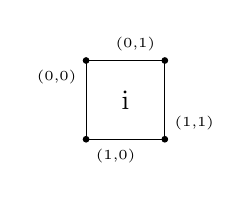
\begin{tikzpicture}
    \draw (0,0) -- (0,1) -- (1,1) -- (1,0) -- (0,0);
    \filldraw[black] (0,1) circle (1pt) node[below left] {\tiny (0,0)};
    \filldraw[black] (1,1) circle (1pt) node[above left] {\tiny (0,1)};
    \filldraw[black] (1,0) circle (1pt) node[above right] {\tiny (1,1)};
    \filldraw[black] (0,0) circle (1pt) node[below right] {\tiny (1,0)};
    \node at (0.5,0.5) {i};
  \end{tikzpicture}
  \caption{Description of the bottom corners position}
  \label{fig:M1}
\end{figure}

The following additional variables are defined:
\begin{table}[hbt!]
  \begin{tabular}{|p{0.1\textwidth}|p{0.85\textwidth}|}
    \hline
    \multicolumn{2}{|l|}{\textbf{Variables}}                                                                                                                                             \\ \hline
    \(T_{gijl}\)    & Binary variable equal to 1 if RTI \(i\in I\) is directly on top of \(j\in I\) in loading configuration \(l\).                                                      \\[0.5em]
    \(GL_{gil}\)    & Binary variable indicating if container \(i\) is on the ground level on truck \(k\) during time period \(t\).                                                      \\[0.5em]
    \(O_{gijuu'l}\) & Binary variable equal to 1 if the bottom corner \((u,u')\) of container \(i\) is immediately supported by container \(j\) on truck \(k\) during time period \(t\). \\ \hline
  \end{tabular}
\end{table}
\FloatBarrier

Constraints~\eqref{eq:ggz} and \eqref{eq:glz} link the \(z\)-coordinate of container \(i\) with the ground–level variable \(GL_{gil}\):
\begin{align}
  M\Bigl(1-GL_{gil}\Bigr) & \geq PZ_{gil} \quad \forall i \in I,\; t \in T \label{eq:ggz}    \\[0.5em]
  1-GL_{gil}              & \leq M\,PZ_{gil} \quad \forall i \in I,\; t \in T \label{eq:glz}
\end{align}

Constraints~\eqref{eq:zu} and \eqref{eq:zd} imply that for \(O_{gijuu'l}\) to be active, the heights of containers \(i\) and \(j\) must be compatible:
\begin{gather}
  \begin{split}
    PZ_{gil} \leq PZ_{gjl}+\sum_{r \in R}\Bigl(r_{gr}\, HZ_{gjlr}+ q_{gr}\, WZ_{gjlr}+ p_{gr}\, LZ_{gjlr}\Bigr) + (1-O_{gijuu'l})M\\
    \forall i,j\in I,\; i\neq j,\; k\in K,\; (u,u')\in U\times U,\; t \in T \label{eq:zu}
  \end{split}\\[0.5em]
  \begin{split}
    PZ_{gil}+(1-O_{gijuu'l})M \geq PZ_{gjl}+\sum_{r \in R}\Bigl(r_{gr}\, HZ_{gjlr}+ q_{gr}\, WZ_{gjlr}+ p_{gr}\, LZ_{gjlr}\Bigr)\\
    \forall i,j\in I,\; i\neq j,\; k\in K,\; (u,u')\in U\times U,\; t \in T \label{eq:zd}
  \end{split}
\end{gather}

Furthermore, the coordinates of the corner \((u,u')\) of container \(i\) must lie within the \(XY\) projection of container \(j\). Constraints~\eqref{eq:px1} and \eqref{eq:px2} link the \(x\)-dimensions, and constraints~\eqref{eq:py1} and \eqref{eq:py2} link the \(y\)-dimensions. Parameter \(\epsilon\) assures that the corner \((u,u')\) has at least \(\epsilon\) support.
\begin{gather}
  \begin{split}
    PX_{gil}+u\left(\sum_{r \in R}(p_{gr}\, LX_{gilr}+ q_{gr}\, WX_{gilr}+ r_{gr}\, HX_{gilr})\right) + M(1-O_{gijuu'l})\\
    \geq PX_{gjl} + \epsilon\, u \quad \forall i,j\in I,\; i\neq j,\; k\in K,\; (u,u')\in U\times U,\; t \in T \label{eq:px1}
  \end{split}\\[0.5em]
  \begin{split}
    PX_{gil}+u\left(\sum_{r \in R}(p_{gr}\, LX_{gilr}+ q_{gr}\, WX_{gilr}+ r_{gr}\, HX_{gilr})\right)
    \leq PX_{gjl}+\sum_{r \in R}(p_{gr}\, LX_{gjlr}+ q_{gr}\, WX_{gjlr}+ r_{gr}\, HX_{gjlr})\\
    + M(1-O_{gijuu'l}) - (1-u)\epsilon \quad \forall i,j\in I,\; i\neq j,\; k\in K,\; (u,u')\in U\times U,\; t \in T \label{eq:px2}
  \end{split}\\[0.5em]
  \begin{split}
    PY_{gil}+u'\left(\sum_{r \in R}(q_{gr}\, WY_{gilr}+ p_{gr}\, LY_{gilr}+ r_{gr}\, HY_{gilr})\right) + M(1-O_{gijuu'l})\\
    \geq PY_{gjl} + \epsilon\, u' \quad \forall i,j\in I,\; i\neq j,\; k\in K,\; (u,u')\in U\times U,\; t \in T \label{eq:py1}
  \end{split}\\[0.5em]
  \begin{split}
    PY_{gil}+u'\left(\sum_{r \in R}(q_{gr}\, WY_{gilr}+ p_{gr}\, LY_{gilr}+ r_{gr}\, HY_{gilr})\right)
    \leq PY_{gjl}+\sum_{r \in R}(q_{gr}\, WY_{gjlr}+ p_{gr}\, LY_{gjlr}+ r_{gr}\, HY_{gjlr})\\
    + M(1-O_{gijuu'l}) - (1-u')\epsilon \quad \forall i,j\in I,\; i\neq j,\; k\in K,\; (u,u')\in U\times U,\; t \in T \label{eq:py2}
  \end{split}
\end{gather}

Constraint~\eqref{eq:4corners} ensures that either a used container is at the bottom of the truck or all four bottom corners are supported by other boxes:
\begin{align}
  \sum_{j\in I,\; (u,u')\in U\times U} O_{gijuu'l} + M\Bigl(GL_{gil}+1-X_{gil}\Bigr) \geq 4 \quad \forall i\in I,\; k\in K,\; t \in T \label{eq:4corners}
\end{align}

Constraint~\eqref{eq:oe} limits \(O_{gijuu'l}\) to be active only if container \(j\) is used during planning period \(t\):
\begin{align}
  O_{gijuu'l} \geq X_{gjl} \quad \forall g \in G,\; i,j\in I,\; (u,u')\in U\times U,\; k\in K,\; t\in T \label{eq:oe}
\end{align}

Additionally, to allow only 90 degree rotations along the \(z\)-axis the following constraint is added:
\begin{align}
  HZ_{gilr}\leq X_{gilr} \quad \forall g\in G,\; r\in R,\; i\in I,\; k\in K,\; t \in T
\end{align}

Finally, the following equations link the RTI stacking variables:
\[
  4\,T_{gijl} = \sum_{(u, u') \in U \times U} O_{gijuu'l} \quad \forall g\in G,\; i,j \in I,\; l \in L,\; i\neq j
\]
\[
  \sum_{j \in I} T_{gijl} \leq 1 \quad \forall g \in G,\; i \in I,\; l \in L
\]



\section{Matheuristic Procedure}
\color{black}
As previously mentioned, exact methods provided by MILP solvers fall short for tackling real world instances with the current computation technology.
Therefore, a matheuristic approach is proposed, Math-3D-SCPTOP. It is based on decoupling the two sub-processes involved in the problem: finding 3D loading configurations of RTIs inside the trucks and determining the number of trucks and what to carry in each time period in order to minimize inventory and transport costs.



This matheuristic is based on two main components.
First a MILP model is defined to determine which loading configurations from a given set should be used in order to minimise the transport and inventory costs. Second a metaheuristic approach is used to identify these loading configurations.

\subsection{PLC-SCPTOP}
The following MILP model, dubbed as PLC-SCPTOP, uses predefined loading configurations of container types to determine which loading configurations to use, the products to carry and the number of trucks in order to minimise inventory and transport costs.
The predefined loading configurations must already obey the spatial constraints defined in 3D-SCPTOP.
Theoretically, if every conceivable loading configuration were incorporated into the model, the optimal solution of PLC-SCPTOP would align with that of 3D-SCPTOP.
Enumerating all of the possible loading configurations of a 3D Bin Packing Problems would take an exponential number of memory space and cpu time with respect the number of container types.
Moreover, solving the PLC-SCPTOP would become even more time-consuming, assuming the MILP program could be fully allocated in memory.

Table \ref{tab:NomenclaturePLC}
\begin{longtable}[hbt!]{  |p{0.07\textwidth}|p{0.8\textwidth}  |}
  \caption{Nomenclature of Math-3D-SCTOP}
  \label{tab:NomenclaturePLC}
  \\
  \hline
  \multicolumn{2}{|l|}{\textbf{Indices}}                                                                                                                                 \\ \hline
  $R$                & Set of RTI types $(r = 1, \dots, R)$                                                                                                              \\
  $K$                & Set of trucks $(k =1,2,\dots , K)$
  \\
  \textit{N}         & Set of products \textit{(n }=   1,…,\textit{N)}                                                                                                   \\
  $L$                & Set of loading configurations $(l =1,2,\dots , L)$
  \\
  \textit{T}         & Set of planning periods \textit{(t} =1, 2…\textit{T)}                                                                                             \\
  $G$                & Set corresponding to the supplier and plant nodes $G = \lbrace s, p \rbrace$                                                                      \\
  \hline
  \multicolumn{2}{|l|}{\textbf{Set of indices}}                                                                                                                          \\ \hline
  $M(r)$             & Set of RM or AP that are carried in RTI $r \in R$, $n = 1, \dots, M(r)$                                                                           \\
  \hline
  \multicolumn{2}{|l|}{\textbf{Parameters}}                                                                                                                              \\ \hline
  $cK$               & Cost of using a truck                                                                                                                             \\
  $lt$               & Lead transport time between the plant and the supplier and viceversa.                                                                             \\
  \textit{$i_{gn}$}  & Initial inventory level of $n\in N$ in $g \in G$ in terms of full RTIs                                                                            \\
  \textit{$ie_{gr}$} & Initial inventory level of empty RTIs $r\in R$ in $g \in G$ RTIs                                                                                  \\
  \textit{$ic_{gn}$} & Inventory cost of $n\in N$ at $g \in G$ in terms of full RTIs                                                                                     \\
  $d_{gnt}$          & Production plan of $n \in N$ at $g \in G$ during time period $t\in T$                                                                             \\
  $q_{rt}$           & Initial quantity of empty RTIs $r\in R$ arriving at supplier $s\in G$ in time period $t \in (1,\dots , lt)$                                       \\
  $q_{nt}$           & Initial quantity of full RTIs of $n \in R$ arriving at $p$ in time period $t \in (1,\dots , lt)$                                                  \\
  $lc_{lrg}$         & Number of containers of type $c$ used in loading configuration $l$ arriving at $g\in G$                                                           \\
  $ss_{gnt}$         & Security stock for product $n\in N$  in time period $t \in T$ in $g \in G$ in terms of full RTIs                                                  \\
  $ss_{gtr}$         & Security stock of empty RTIs $r\in R$  in time period $t \in T$ in $g \in G$                                                                      \\
  \textit{$w_{n}$}   & Weight of a container carrying product \textit{n}
  \\
  $k_t$              & Numbers of trucks available at time period $t$                                                                                                    \\
  \textit{$pK$}      & Maximum  weight capacity of a truck                                                                                                               \\ [0.15cm]
  \hline
  \multicolumn{2}{|l|}{\textbf{Decision Variables}}                                                                                                                      \\ \hline
  $I_{gnt}$          & Inventory of product $n\in N$ at the end of $t\in T$ time period at $g\in G$ in terms of full RTIs                                                \\
  $Ie_{gtr}$         & Inventory of empty RTIs $r\in R$ at the end of $t\in T$ time period at $g\in G$                                                                   \\
  $Y_{gkt}$          & Binary variable, if one then  truck $k \in K$ is used in time period $t\in T$ arriving at $g\in G$ and zero otherwise                             \\
  $Y_{gklt}$         & Binary variable, if one then truck $k \in K$ is used in time period $t\in T$ departing from $g\in G$ using loading configuration $l$, 0 otherwise \\
  $Q_{nt}$           & Integer variable indicating the number of RM or AP $n\in N$ in transport during time period $t$ to the manufacturing plant $p$                    \\
  $Q_{rt}$           & Integer variable the number of empty RTIs $r\in R$ in transport during time period $t$ to the supplier $s$                                        \\
  $V_{gklrt}$        & Number of RTIs $r\in R$ in truck $k\in K$ using loading configuration $l\in L$ at time period $t\in T$ departing from $g\in G$                    \\
  $V_{kglnt}$        & Number of full RTIs with RM or AP $n\in N$ in truck $k\in K$ using loading configuration $l\in L$ at time period $t\in T$ departing from $g\in G$ \\
  \hline
\end{longtable}


{
We wish to minimise the total cost, which is given by  transportation and inventory costs.}
\begin{equation}
  \text{\textit{Min} } z= \sum_{g \in G}{\sum_{k \in K}{\sum_{t \in T}{Y_{gkt}\cdot cK}}}+ \sum_{g \in G}{\sum_{n \in N}{\sum_{t \in T}{I_{gnt}\cdot ic_{gn}}}}
\end{equation}


\eqref{eq:1PLC} - \eqref{eq:2PLC}  define the inventory level of RM or AP according to the production demand and supply of RM or AP  from the supplier $s$ at the plant  $p$
\begin{align}
  I_{pnt}  & =I_{pnt^{\prime}}-d_{pnt}+Q_{nt^{\prime}}\quad             & \forall n \in N,t \in T : t\ge    lt +1,t^{\prime}\coloneqq t-lt \label{eq:1PLC} \\
  I_{pnt}  & =I_{pnt'}-d_{pnt}+q_{nt}\quad                              & \forall n \in N,t \in (2,\dots, lt) : ,t^{\prime}\coloneqq t-lt\label{eq:3PLC}   \\
  I_{pnt}  & =i_{pn}-d_{pnt}+q_{nt}\quad                                & \forall n \in N: t \coloneqq 1 \label{eq:2PLC}                                   \\
  Ie_{ptr} & =Ie_{pt^{\prime}r}+\sum_{n \in M(r)}{d_{pnt}}-Q_{rt} \quad & \forall r \in R,t \in T : t\ge 2                                                 \\
  Ie_{ptr} & =ie_{pr}+\sum_{n \in M(r)}{d_{pnt}}-Q_{rt}\quad            & \forall r \in R , t\coloneqq 1
\end{align}
\eqref{eq:1PLC-s} - \eqref{eq:2PLC-s}  the empty RTIs according to the production demand and supply of RTIs from the plant $p$ at the supplier $s$
\begin{align}
  I_{snt}  & =I_{snt^{\prime}}+d_{snt}-Q_{nt}\quad                              & \forall n \in N,t \in T,t^{\prime} \in T, : t\ge    2,t^{\prime}\coloneqq t-lt \label{eq:1PLC-s} \\
  I_{snt}  & =i_{sn}+d_{snt}-Q_{nt}\quad                                        & \forall r \in R : t\coloneqq 1 \label{eq:2PLC-s}                                                 \\
  Ie_{str} & =Ie_{st^{\prime}r}+Q_{rt^{\prime}}-\sum_{n \in M(r)}{d_{snt}}\quad & \forall r \in R,t \in T : t\ge    lt +1,t^{\prime}\coloneqq t-lt                                 \\
  Ie_{str} & =Ie_{st^{\prime}r}+q_{rt}-\sum_{n \in M(r)}{d_{snt}}\quad          & \forall r \in R,t \in (2,\dots, lt) : ,t^{\prime}\coloneqq t-lt
  \\
  Ie_{str} & =ie_{pr}+q_{rt}-\sum_{n \in M(r)}{d_{snt}}\quad                    & \forall r \in R:t=1
\end{align}
Each product must satisfy a minimum security stock $ss_{gnt}$.

\begin{equation}
  I_{gnt}\ge ss_{gnt}\quad \forall g \in G,n \in N,t \in T
\end{equation}
\eqref{eq:onelpertPLC} imposes that a truck $k$ can only use one loading configuration $l$ with direction $g\in G $ in time period $t$.
\begin{align}
  \sum_{l\in L}Y_{gklt}=Y_{gkt}\quad \forall k \in K,g \in G,t \in T \label{eq:onelpertPLC}
\end{align}

\eqref{eq:sameasloading1PLC} - \eqref{eq:sameaslaoding2PLC} impose that  the truck $k$ at time period $t$ using loading configuration $l$ uses the same loading configuration as $l$.
\begin{align}
  V_{gklrt} & +M\cdot (1-Y_{gklt})\ge lc_{lrg}               & \quad \forall k \in K,g \in G,l \in L,t \in T\label{eq:sameasloading1PLC} \\
  V_{gklrt} & \le Y_{gklt}\cdot lc_{lrg}+M\cdot (1-Y_{gklt}) & \quad \forall k \in K,l \in L,g \in G,t \in T\label{eq:sameaslaoding2PLC}
\end{align}

Since a product can only be carried by one container type \eqref{eq:numnpercPLC} sets that the number of containers of type $c$ carried at truck $k$ using loading configuration $l$ at time period $c$ is equal to the sum of containers carried of products $n$ which containers of type $c$ can carry. Moreover, \eqref{eq:amountnattPLC} sets the total amount of product $n$ being transported from $s$ to $p$ in time period $t$, and \eqref{eq:amountnattPLC2} sets the total amount of RTIs $r$ being transported from $p$ to $s$ in time period $t$,
\begin{align}
  V_{pklrt} & =\sum_{n \in M(r)}{V_{pklnt}}\quad              & \forall k \in K,l \in L,t \in T,r \in R \label{eq:numnpercPLC} \\
  Q_{nt}    & =\sum_{l \in L}{\sum_{k \in K}{V_{kslnt}}}\quad & \forall n \in N,t \in T\label{eq:amountnattPLC}                \\
  Q_{rt}    & =\sum_{l \in L}{\sum_{k \in K}{V_{pklrt}}}\quad & \forall r \in R,t \in T\label{eq:amountnattPLC2}
\end{align}


\eqref{eq11PLC} guarantees that the maximum weight allowed for truck \textit{k} is not surpassed.

\begin{align}
   & \sum_{l,n} w_{n}V_{kglnt} \leq pK & \forall k\in K,t\in T, g \in G \label{eq11PLC}
\end{align}

\begin{align*}
  I_{gnt}   & \in \mathbb{Z}_{\geq 0} \quad &  & \forall g \in G,\; n \in N,\; t \in T,                       \\
  Ie_{gtr}  & \in \mathbb{Z}_{\geq 0} \quad &  & \forall g \in G,\; t \in T,\; r \in R,                       \\
  Y_{gkt}   & \in \{0,1\} \quad             &  & \forall k \in K,\; g \in G,\; t \in T,                       \\
  Y_{gklt}  & \in \{0,1\} \quad             &  & \forall k \in K,\; g \in G,\; l \in L,\; t \in T,            \\
  Q_{nt}    & \in \mathbb{Z}_{\geq 0} \quad &  & \forall n \in N,\; t \in T,                                  \\
  Q_{rt}    & \in \mathbb{Z}_{\geq 0} \quad &  & \forall r \in R,\; t \in T,                                  \\
  V_{gklrt} & \in \mathbb{Z}_{\geq 0} \quad &  & \forall g \in G,\; k \in K,\; l \in L,\; r \in R,\; t \in T, \\
  V_{kglnt} & \in \mathbb{Z}_{\geq 0} \quad &  & \forall k \in K,\; g \in G,\; l \in L,\; n \in N,\; t \in T.
\end{align*}


\subsection{Meta-Heuristic Procedure}
The objective of the metaheuristic is to obtain good loading configurations so the PLC-SCPTOP model can optimise transport and inventory costs while managing RTI flow. Therefore, the metaheuristic should consider the temporal nature of the problem. That is, the loading problem must consider the future demand of products and the current state of inventories.

To simulate the production and transportation, we define two separate processes. On the one hand, we have the plant processes and on the other we have the supplier processes. In each node, we first receive the RTIs, then we produce, and after that we make the transport decisions. \ref{fig:Procceses} illustrates the both processes and the connections between them.

\begin{figure}[!h]
  \centering
  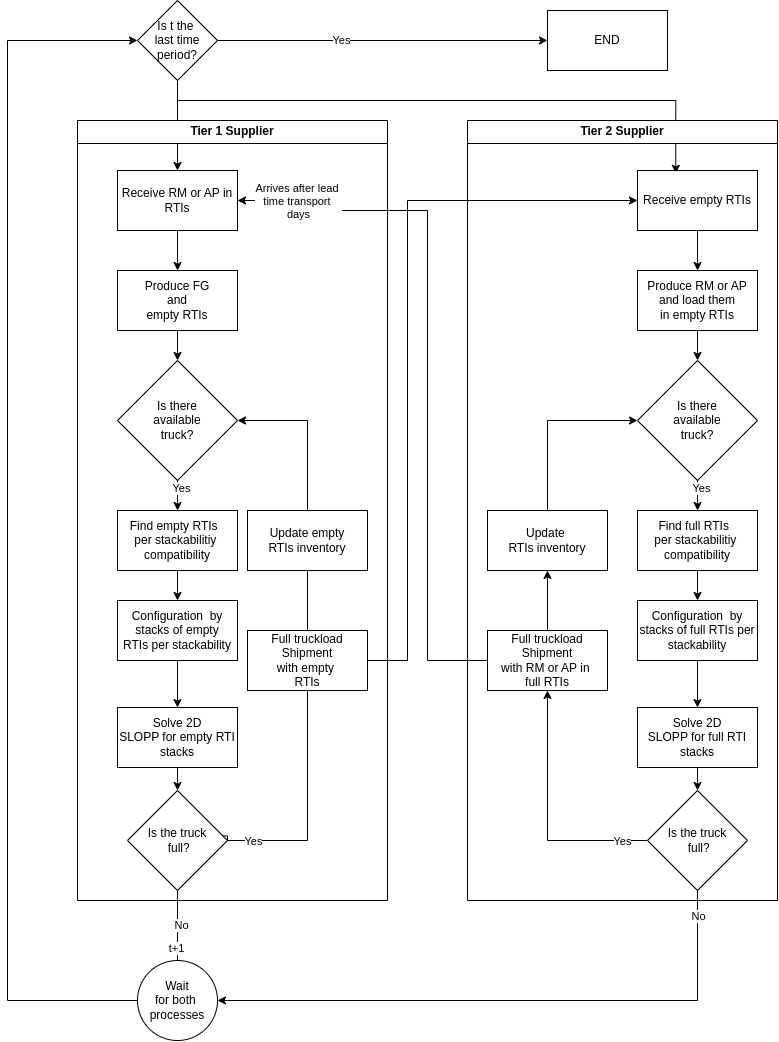
\includegraphics[width=0.75\linewidth]{figures/image.png}
  \caption{Procceses of plant and supplier}
  \label{fig:Procceses}
\end{figure}

In both cases, we need to determine transport decisions. That is, the loading configurations and what is going to be transported. We can only transport what we already have in stock. Furhtermore, RTIs are loaded into the truck as stacks. Each RTI has a set of compatible RTIs which can be stacked with. We use a column generation technique to find the RTIs stacks that can be loaded. Then, we find a loading configuration through a 2D-SLOPP formulation, where the stacks that contain RTIs needed in the other supply chain node for the next products are prioritized through the objective function. Once the RTI loading configuration is determined, we decide RM or AP procurement for the manufacturing site, prioritizing RMs or APs which have less stock at the manufacturing site.

\begin{algorithm}[h!]
  \caption{Loading Configurations}\label{alg:MITP}
  \begin{algorithmic}
    \Procedure{LoadingConfigurations}{}
    \State $T$ \# List of time periods
    \State LC=[] \# List of loading configurations
    \For{ $t\in T$}
    \For{ $\delta \in  \Delta$ }
    \State IncomingTransport(t)

    \State Produce(t)
    \While {TransportResourceAvailable}
    \State C = ContainersToLoad(t, $\delta$, LC)
    \State
    \State
    \State LC.append(PackContainers(C,t))
    \EndWhile
    \EndFor
    \EndFor
    \State LC=EliminateDuplicateOrDominatedLoadingConfigurations(LC)
    \State \textbf{return} LC
    \EndProcedure
  \end{algorithmic}
\end{algorithm}

We will use the previously found loading configurations to consider the time dependency of the loading problem at hand. For each period $t\in T$, we will solve the PLC-SCPTOP problem from day 1 to $t$ with the current loading configurations obtained to find the inventory levels of the products at day $t$. Then, we find the necessary containers for the following $\delta \in \Delta$ days, where $\Delta$ is a user-defined list of parameters.


\begin{algorithm}[h!]
  \caption{Final Loading Configurations}\label{alg:MITP2}
  \begin{algorithmic}
    \Procedure{Final Loading Configurations(LC)}{}
    \State TimePeriods \# List of time spans to calculate the number of needed products
    \State TimeSpan \# List of time spans to calculate the number of needed products
    \For{ t $in$ TimePeriods}
    \For{ $\delta$ in TimeSpan}
    \State I=SolvePLC-SCPTOP(LC,t)
    \State C= ContainersToLoad(I,t, $\delta$, LC)
    \State LC.append(PackContainers(C,t))
    \EndFor
    \EndFor
    \State LC=EliminateDuplicateOrDominatedLoadingConfigurations(LC)
    \State \textbf{return} LC
    \EndProcedure
  \end{algorithmic}
\end{algorithm}




Finally, we feed the loading configurations found by Algorithms \ref{alg:MITP} and \ref{alg:MITP2} to the PLC-SCPTOP mathematical modelling as parameters to find reasonable quality solutions to 3D-SCPTOP problem.

\begin{algorithm}
  \caption{MathH-3D-SCPTOP}
  \begin{algorithmic}[1]
    \State $\Delta_1, \Delta_2$ \# List of time spans to calculate the number of needed products
    \State LC = InitialLoadingConfiguration($\Delta_1$)
    \State LC = FinalLoadingConfiguration(LC, $\Delta_2$)
    \State SolvePLCSCPTOP(LC,$|$T$|$))
  \end{algorithmic}
\end{algorithm}

\subsubsection{Loading Procedure}

To address the loading problem, will divide the problem in two parts. First, we will find through a column generation technique for the cutting stock problem to find different stacks that will be loaded. Once these stacks are found, we will

\section{Computational and comparative analysis}
Here the 3D-SCPTOP model is validated and compared to the work by \autocite{Diaz-Madronero2014APlanning}.  This fuzzy optimisation model integrates procurement transport and inventory holding decisions by contemplating transport capacity restrictions by a maximum number of containers per truck, which we refer to as SCPTOP from this point onwards. To compare the SCPTOP model, we make three key modifications: fuzzy parameters are not considered; transport capacity restriction takes into account the volume of individual containers and the truck’s capacity; products can be loaded in more than one container type. The SCPTOP model is extended and defined in Appendix \ref{appendix:A}.
We evaluate and compare both the 3D-SCPTOP and SCPTOP models, in terms of solution quality, transport costs, inventory costs and computational times. The 3D-SCPTOP and SCPTOP mathematical formulations are solved for all the instance sets with CP-SAT from OR-Tools and Gurobi using their default settings. Additionally, as $(C\& P)$ problems are NP-hard, the Meta-3D-SCPTOP algorithm has been developed to find igh-quality solutions for large real-world instances, based on a case study. So the performance of the 3D-SCPTOP, the Meta-3D-SCPTOP and the SCPTOP models is compared and evaluated as follows.


Twenty-four instances are artificially generated by a stochastic process, whose key characteristics are given as follows:

\begin{itemize}
  \item \textbf{Demand Generation}: the demand for each product is randomly generated by deviating from a given mean by plus or minus ten percent. This introduces variability into the demand values for different products

  \item \textbf{Time Periods}: Half of the instances have a total of five time periods, while the other half have a total of ten time periods. This allows evaluating the model's performance over different time horizons.

  \item \textbf{Container Types}: Each instance includes a varying number container types, specifically two, three or four. The distribution of container types is the same among instances, which implies that an equal number of instances has the same number of containers

  \item \textbf{Container Dimensions}: The dimensions of each container type are randomly generated. The width, length and height of boxes are fractions of the width, length, or height of trucks. This randomness ensures diversity in the sizes of containers across the generated instances. An additional constraint is applied to the generation of containers. The volume of each container must be at least 1/n of the truck’s volume, where n can take the values of four, six or eight. This ensures that containers are appropriately sized in relation to trucks

\end{itemize}
By incorporating these stochastic elements into the generation process, the 24 instances provide a diverse set of scenarios for evaluating the model’s performance. Variability in demand, time periods, box types and box dimensions introduces realistic and challenging conditions that the model needs to address. Furthermore, we use the number of time periods, the number of box types, the number of products and the maximum amount of containers needed to load a truck (in volume terms) as explanatory variables of various metrics from the models, such as total cost, transport cost, inventory cost, solution gap and solution time. The instance name is in the form of \textit{I\_n\_t\_c\_v}, where n is product type, t is the number of time periods, c is the number of container types and v is the minimum volume of containers.

Each test is limited to 4 hours (14,400 seconds) of run-time per instance. Tests are performed on a Microsoft Windows Server 2022 Standard n with an AMD EPYC 7402 24-Core Processor running at 2,800 MHz, with 256 GB of RAM using Python as the programming language.



\section{Practical application}

This section presents a practical procurement transport application. The proposed resolution framework was evaluated using real data from an automotive industry supply chain. We validate and compare the 3D-SCPTOP solution procedures to the company’s procedure, which employs predefined loading configurations that indicate the number of each container type to be carried. Finding these loading configurations is a very tedious and time-consuming manual task that is based on a spreadsheet procedure. A mathematical programming model, dubbed as PLC-SCPTOP, which replicates the current’s company procedure, is then utilised to minimise the total cost, with a summation of procurement transport and inventory holding costs, and one based on these predetermined configurations.




The real-world data derived from the company’s operations act as the empirical foundation for examining both the PLC-SCPTOP and the Meta-3D-SCPTOP. To broaden the scope of this analysis, we scale and manipulate these data, guided by a stochastic process, to simulate several potential operational scenarios. Setting our analysis to mirror the dynamic and unpredictable realities of supply chain operations thus enhances the validity of our evaluation and the practical relevance of the suggested metaheuristic. For this purpose, we propose three different scenarios for the created instances: normal demand, low variability demand, high variability demand. Table \ref{tab:ResultsFromCaseStudy}, found in the Appendix \ref{appendix:A}outlines the models’ performance across these instances. Table \ref{tab:CaseStudySumary} summarises models’ performance and resolution times.

\begin{table}[h!]
  \centering
  \caption{Summary of performance for the practical application}
  \label{tab:CaseStudySumary}
  \begin{adjustbox}{angle=0}
    \centering
    \begin{tabular}{lrrr}
      \toprule
      Model          & Objective Value & Best Bound    & Duration (seconds) \\
      \midrule
      MathH-3D-SCTOP & 252235.198934   & 247307.820849 & 740.000000         \\
      Meta-3D-SCTOP  & 256715.145777   & NaN           & 677.555556         \\
      PLC-SCTOP      & 275226.680415   & 271798.477640 & 44.670370          \\
      \bottomrule
    \end{tabular}
  \end{adjustbox}
\end{table}

Figures \ref{fig:a1} - \ref{fig:a2} describe the performance of both the models and solution procedures in the different scenarios. The x-axis shows the scenario, while the y-axis depicts the objective value, inventory costs, or transport costs. Each colour represents a different model applied to obtain the solution.


The results reveal that an effective systematic method is proposed for solving procurement transport operational planning with 3D full-truck loading constraints. This solution is both automated and executed within a reasonable computational timeframe. Our methodology proves particularly beneficial when there is significant discrepancy between the company’s proposed loading configurations and the actual demand concerning container types. In such instances, the company is usually left with two choices: either use the fixed loading configurations and, thus, incur higher inventory and transport costs, or manually resolve the loading configuration via a spreadsheet procedure, which might lead to errors. However, one potential disadvantage of the proposed Meta-3D-SCPTOP is its performance under normal demand conditions because the demand for different container types is consistent with the loading configurations, but the metaheuristic may result in fewer optimal inventory holding costs compared to the company’s current procedure. This is because the Meta-3D-SCPTOP obtains decisions locally, while exact methods are guaranteed, given enough time, to find the optimal solution.

This issue is, however, solved when utilising MathH-3D-SCPTOP because it effectively combines both heuristic and exact methods. While the heuristic provides a fast and reasonably good solution for the initial loading configurations, the exact method improves it by further lowering inventory and transport costs.

Therefore, this method shows promising results for reducing inventory and transport costs, particularly under variable demand and misalignment between loading configurations and container types.
\section{Conclusions}
We herein propose a MILP model, 3D-SCPTOP, to tackle procurement transportation planning at an operational level by incorporating 3D loading constraints into its considerations. Given the NP-hard nature of 3D bin packing, we have also developed a metaheuristic approach, Meta-3D-SCPTOP, which is later refined and enhanced by employing a mathheuristic technique, MatH-3D-SCPTOP.

A case study has also been conducted within an automotive SC that comprises a car assembler, a first-tier supplier and a second-tier supplier. The objective of the 3D-SCPTOP model is twofold: (i) to minimise the total number of trucks used; (ii) to minimise inventory holding costs. This approach takes into account the complexities of supply chain logistics in the automotive industry by demonstrating a successful integration of procurement transport planning and 3D loading constraints.

Managerial implications in a SC context are oriented to the proposed solution methodology, improving the solutions found by the company’s procedure. It is also able to adapt to demand changes while finding high-quality solutions in reasonable computational times.

Nevertheless, several challenges remain for further research lines to deal with; for instance, the inclusion of multiple suppliers to better represent complex supply chains. A more comprehensive transport operation model could be achieved by incorporating routing aspects, such as vehicle routing with 3D loading constraints. Furthermore, the introduction of dynamic stability into loading constraints may also yield more practical, robust solutions. Integrating sourcing and delivery transport decisions could improve supply chain efficiency. Finally, the incorporation of production scheduling into the model has the potential of offering a cohesive approach to supply chain planning optimisation by aligning production timelines with transportation and inventory strategies.


% \input{vistex/MF2}


\FloatBarrier
\begin{ChapterAppendix}
  
\section{Mathematical Model}

\label{appendix:A}
\FloatBarrier
\begin{table}
  \caption{Nomenclature of Supply Chain Operation Transport Planning}
  \begin{tabular}{|c|c|}
    \hline \multicolumn{2}{|c|}{ Sets of indices }                                                                \\
    \hline I:             & Set of products $(i=1,2, \ldots, I)$                                                  \\
    \hline$J:$            & Set of groups composed of products that must be ordered together $(j=1,2, \ldots, J)$ \\
    \hline$K:$            & Set of trucks $(k=1,2, \ldots, K)$                                                    \\
    \hline$T:$            & Set of planning periods (days) $(t=1,2, \ldots, T)$                                   \\
    \hline \multicolumn{2}{|c|}{ Decision variables }                                                             \\
    \hline$Q_{i k t:}$    & Units transported of $i$ by $k$ in period $t$ (units)                                 \\
    \hline$G_{i j k t}$ : & Units transported of $i$ corresponding to group $j$ by $k$ in period $t$ (units)      \\ \hline
    { $C_{k t}:$}         & {Volume of containers transported by $k$ in period $t$ (units)}                       \\
    \hline$I_{i t}:$      & Inventory amount of $i$ at the end of period $t$ (units)                              \\
    \hline$K_{j k t:}$    & Number of lots to order of products of group $j$ by $k$ in period $t$                 \\
    \hline$Y_{k t}$       & Binary variable indicating whether a truck $k$ has been used in period $t$            \\
    \hline \multicolumn{2}{|c|}{ Objective functions }                                                            \\
    \hline$z_1:$          & Total number of trucks utilized                                                       \\
    \hline$z_2$           & Total inventory amount generated                                                      \\
    \hline \multicolumn{2}{|c|}{ Parameters }                                                                     \\
    \hline$u_i:$          & Amount of product $i$ that fits in a container (units)                                \\
    \hline$l_j:$          & Number of units of each group lot $j$ (units)                                         \\
    \hline$b_{i j}$       & 1 if product $i$ belongs to group $j$, and 0 otherwise                                \\
    \hline$D_{i t}:$      & Demand of product $i$ in $t$ (units) (considered firm)                                \\
    \hline$\Gamma_k:$     & Volume of truck \textit{k}                                                            \\
    \hline$\Gamma_i:$     & Volume of container carrying product \textit{i}                                       \\
    \hline $\mathrm{m}:$  & Minimum truck occupation (in containers)                                              \\
    \hline $I0_i$         & Inventory amount of $i$ in period 0                                                   \\
    \hline $IC_i$         & Inventory cost of $i$                                                                 \\
    \hline $C_k$          & Cost of using truck k                                                                 \\
    \hline $SC_i$         & Number of days of stock coverage for product i
    \\
    \hline
  \end{tabular}
\end{table}
\FloatBarrier
Minimize the total cost transport and inventory
$$
  \operatorname{Min} z \cong \sum_{k=1}^K \sum_{t=1}^T Y_{k t} + \sum_{i=1}^I \sum_{t=1}^T I_{i t}\cdot IC_i
$$
subject to
$$
  \begin{aligned}
     & I_{i t}=I_{i(t-1)}-D_{i t}+\sum_{k=1}^K Q_{i k t} \quad \forall i\in I, t \in  T,                                                               \\
     & Q_{i k t}=\sum_{j=1}^J G_{i j k t} \quad \forall i \in I, k \in K, t \in T,                                                                     \\
     & G_{i j k t}=K_{j k t} \cdot l_j \cdot b_{i j} \quad \forall i \in I, j \in I, k\in K, t \in T,                                                  \\
     & C_{k t}=\sum_{i=1}^l Q_{i k t} / u_i \cdot \Gamma_i \quad \forall k \in K, t \in T,                                                             \\
     & C_{k t} \leqslant \Gamma_k \cdot Y_{k t}\quad \forall k \in K, t \in T,                                                                         \\
     & C_{k t} \geqslant m \cdot \Gamma_k Y_{k t} \quad \forall k \in K, \in T                                                                         \\
     & I_{n t }\geq     \begin{cases}
                          \sum_{s \in \lbrace 1 , \dots , SC_i \rbrace } D_{i,t+s} \quad  & \text{if } i\in I, t \in \lbrace 1, \dots , |T|-SC_i \rbrace \\
                          \sum_{s \in \lbrace 1 , \dots , SC_i \rbrace } D_{i,|T|-SC_i+s} & \text{ other wise }
                        \end{cases} \\
     & Y_{k t} \leqslant 1 \quad \forall k, t,                                                                                                         \\
     & I_{i t}, Q_{i k t}, G_{i j k t}, C_{k t}, K_{j k t}, Y_{k t} \geqslant 0 \text { integer } \quad \forall i \in I, j \in I, k \in K, t \in T .
  \end{aligned}
$$
In our case $|J|=|I|$, one group for each product.

\end{ChapterAppendix}
